% !TEX encoding = UTF-8 Unicode
% !TEX root =  ../Bachelorarbeit.tex

\chapter{\"Uberblick}
\label{sec:UeberblickEntwicklungsplattform}

Die gew\"ahlte Entwicklungsplattform ist entscheidend f\"ur die darauf folgende Implementierung eingebetteter Software. Im Rahmen dieser Arbeit dient der MSP430FR5729 von Texas Instruments als zentrale Hardwarekomponente. Dessen Technische Daten und Funktionalit\"aten werden in den folgenden Abschnitten n\"aher betrachtet.

Der MSP430FR5729 ist ein Low-Power-Microcontroller  \Fachbegriff{Mikrocontroller mit 16-Bit-Registerbreite und reduzierter Befehlssatzarchitektur (Reduced Instruction Set Computer)}{16-Bit-RISC-Microcontroller} von Texas Instruments mit einer Maximalen Taktfrequenz von Acht \Fachbegriff{Ma{\ss}einheit f\"ur die Frequenz und entspricht einer Million Schwingungen pro Sekunde (1 MHz = 10$^{6}$ Rechenschritte).}{Megaherz}. Eingebaute Low-Power-Modi (\Abkuerzung{Low Power Mode}{LPMs}[LPM]) erm\"oglichen \ua niedrigere Taktfrequenzen und das deaktivieren von Oszillatoren, wodurch er sich besonders gut f\"ur energieeffiziente Anwendungen im Bereich eingebetteter Systeme eignet. Eine Auflistung aller Modi sind in \Abbildung{operation_modes} zu sehen. \Zitat[S. 43, Kap. 6.3, S. 35, Kap. 1.4 \& S. 37, Kp. 1.4.1]{ti:slase35c, ti:slau272d}

\begin{figure}[h!]
	\centering
	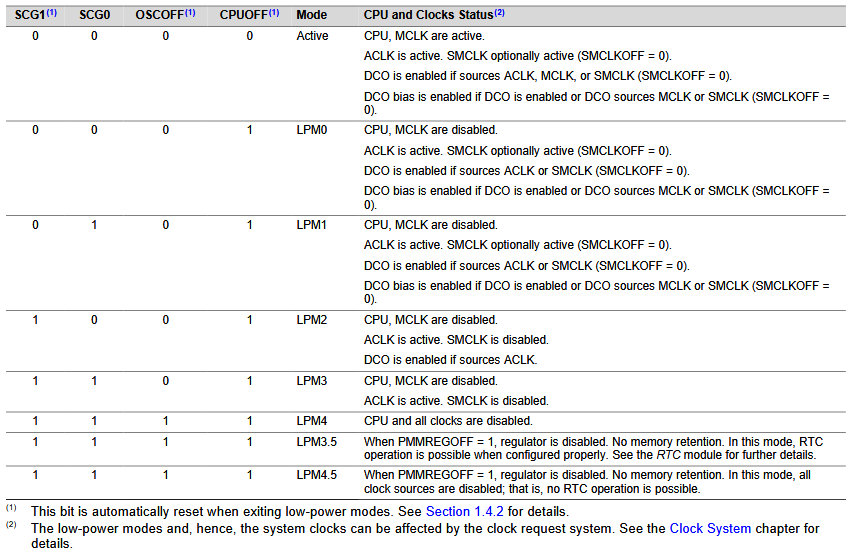
\includegraphics[width=1.0\textwidth]{../Bilder/Operating_Modes.png}
	\caption{Operating Modes \Zitat[S. 37, Kap. 1.4, Tab. 1-2]{ti:slau272d}}
	\label{fig:operation_modes}
\end{figure}

Der Mikroprozessor besitzt 16 Kilobyte an nicht-fl\"uchtigen FRAM, sowie ein Kilobyte \Fachbegriff{Schnellster, fl\"uchtiger Speicher mit geringer Kapazit\"at, bestehend aus Flip-Flops welcher meist direkt in der \Abkuerzung{Central Processing Unit}{CPU} mit eingebaut ist.}{statischen Arbeitsspeicher}[statischer Arbeitsspeicher] (\Abkuerzung{Static Random Access Memory}{SRAM}). 

Die Versorgungsspannung betr\"agt 2 bis 3,6 Volt wobei ebenfalls verschiedene Low-Power-Modi verwendet werden k\"onnen, um den Stromverbrauch zunehmend zu minimieren. Diese beeinflussen den sp\"ateren Umgang mit Timer-Interrupts, weil sie den Energieverbrauch im Wartezustand beeinflussen. \Zitat[S. 26, Kap. 5.20]{ti:slase35c}

Des Weiteren besitzt der Chip F\"unf Interne 16-Bit Timer mit jeweils Sieben\\\NeuerBegriff{Capture and Compare} Registerbl\"ocken. Diese internen Timer stellen eine zentrale Komponente f\"ur die Realisierung pr\"aziser Zeitgesteuerter Funktionen und die Generierung von Interrupts dar, welche im nachfolgenden \Kapitel{TIMER&ISR} tiefgreifender erl\"autert werden.

Zur externen Kommunikation sind Protokolle wie \Abkuerzung{Universal Asynchronous Receiver Transmitter}{UART}, \Abkuerzung{Inter-Integrated Circuit}{I$^{2}$C} und \Abkuerzung{Serial Peripheral Interface}{SPI} integriert, welche mit 32 Programmierbaren \Abkuerzung{General Purpose Input/Output}{GPIO}-Pins angeschlossen werden k\"onnen. Kommunikationsschnittstellen sind f\"ur die Interaktion mit der Au{\ss}enwelt und Peripherieger\"aten von hoher Bedeutung. Eine detailliertere Ausarbeitung des \Fachbegriff{Serielle Schnittstelle in Mikrocontrollern von Texas Instruments, die verschiedene Kommunikationsprotokolle (\zB UART, SPI, I$^{2}$C) unterst\"utzt.}{enhanced Universal Serial Communication Interface} (\Abkuerzung{enhanced Universal Serial Communication Interface}{eUSCI}) folgt in \Kapitel{eUSCI}. \Zitat[S. 1, Kap. 1.1]{ti:slase35c}

\begin{figure}[h!]
	\centering
	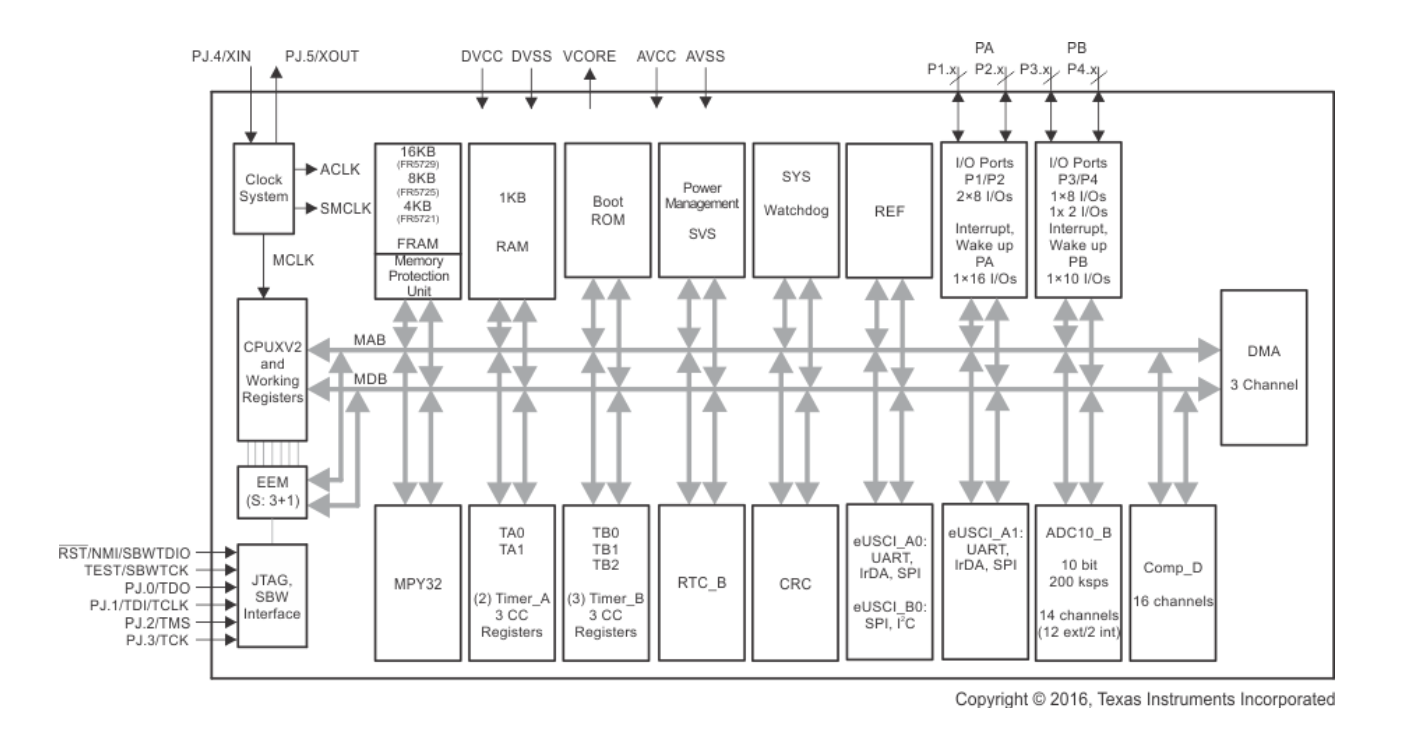
\includegraphics[width=1.0\textwidth]{../Bilder/FunctionalBlockDiagram_MSP430FR5729.png}
	\caption{Block Diagramm MSP430FR5729\\Mikrocontroller \Zitat[S. 2, Kap. 1.4]{ti:slase35c}}
	\label{fig:BlockDiagramm_msp430}
\end{figure}

\newpage
\Abbildung{BlockDiagramm_msp430} zeigt ein vollst\"andiges Block-Diagramm des Mikroprozessors, welches noch einige weitere Eigenschaften, Funktionen und Subsysteme auflistet. \AI


\section{Timer und Interrupt Service Routinen (ISR)}
\label{sec:TIMER&ISR}

Timer und Interrupt Service Routinen (\Abkuerzung{Interrupt Service Routine}{ISR\grq s}[ISR]) stellen einen fundamentalen Baustein moderner eingebetteter Systeme dar. Sie erm\"oglichen pr\"azise, zeitgesteuerte Funktionen als auch das reagieren auf externe Ereignisse. Womit die Realisierungen komplexer, Echtzeitsysteme m\"oglich wird. Im Folgenden wird die Timer-Architektur des MSP430FR5729 und die zugeh\"origen ISR-Mechanismen detailliert betrachtet.

Der MSP430FR5729 verf\"ugt \"uber insgesamt f\"unf 16-Bit-Timer, wovon zwei zu Typ A und drei zu Typ B geh\"oren. Timer haben vielseitige Einsatzgebiete und erm\"oglichen verschiedenste Zeitsteuerungsfunktionen. Die Unterscheidung in zwei Typen l\"asst dabei eine gr\"o{\ss}ere Vielfalt an spezifischen Konfigurationsm\"oglichkeiten zu.

\newpage
Beide Timer-Typen verf\"ugen \"uber einen gemeinsamen 16-Bit-Z\"ahler sowie sieben Capture/Compare-Register. Die korrekte Konfiguration dieser Register ist ausschlaggebend f\"ur die Implementierung verschiedenster Funktionen. Eine der beiden \"ubergeordneten Eigenschaften, die Capture-Funktionalit\"at, dient dazu, den aktuellen Z\"ahlerwert bei einem externen oder internen Ereignis pr\"azise zu erfassen. Dies ist beispielsweise n\"utzlich f\"ur die Messung von Pulsweiten oder Frequenzen. Die Compare-Funktionalit\"at hingegen erlaubt den Vergleich des aktuellen Z\"ahlerstandes mit einem in den Compare-Registern hinterlegten Wert. Bei einer \"ubereinstimmung kann eine konfigurierbare Aktion ausgel\"ost werden, wie beispielsweise das Setzen oder R\"ucksetzen eines Ausgangspins oder das Generieren eines Interrupts. Ausf\"uhrlicher beleuchtet ab \Kapitel{Timer_CaptureMode}. Die vielseitigen Einstellungsm\"oglichkeiten dieser und weiterer Register erlauben die Realisierung komplexer Zeitgesteuerter Aufgaben. \Zitat[S. 333, Kap. 11 \& S. 355, Kap. 12, S. 287, Kap. 8.3 \& S. 194, Kap. 6.8.2]{ti:slau272d,davies:msp430}

Die Timer des Typs B weisen im Vergleich zu dem Timer des Typs A, erweiterte Konfigurationsm\"oglichkeiten auf. Darunter f\"allt die Konfigurierbarkeit der Timer-L\"ange auf 8, 10, 12 oder 16 Bit, was eine flexible Anpassung der Z\"ahlaufl\"osung und der \"uberlaufperiode f\"ur unterschiedliche Aufl\"osungen erm\"oglicht. Zus\"atzlich sind alle Capture/Compare-Bl\"ocke doppelt gepuffert. Diese doppelte Pufferung erlaubt das Laden neuer Vergleichswerte, w\"ahrend eines aktiven Z\"ahlzyklus. Unerw\"unschte Effekte oder Inkonsistenzen in den Ausgangssignalen k\"onnen dadurch vermieden werden. Ein weiterer Unterschied besteht darin, dass die Capture/Compare-Eing\"ange asynchron zueinander sind. Somit k\"onnen sie unabh\"angig zum internen Takt des Timers operieren, was in bestimmten Szenarien die Erfassung externer Ereignisse erleichtert. \Zitat[S. 356, Kap. 12.1.1, S. 353, Kap. 8.9]{ti:slau272d, davies:msp430}

F\"ur die pr\"azise Steuerung und Ereignisbehandlung bieten die Timer verschiedene Betriebsarten, die im Folgenden n\"aher erl\"autert werden.

\newpage
\subsection{Timer Z\"ahlweisen}
\label{sec:Timer_CountMode}

Der Z\"ahlmodus, bestimmt die interne Z\"ahlweise des Timers. Die Timer unterst\"utzen typischerweise mehrere Varianten, um unterschiedlichen Anforderungen gerecht zu werden. \Zitat[S. 291, Kap. 8.3.1]{davies:msp430}

\begin{itemize}
	\item \textbf{Up Mode:} Im Up Mode (Additive Z\"ahlweise, \Vgl \Abbildung{up_mode}) beginnt der Z\"ahler bei Null und inkrementiert seinen Wert mit jedem Taktimpuls der gew\"ahlten \Fachbegriff{Eine Referenz auf ein periodisches Zeitsignal um zeitliche Abl\"aufe zu synchronisieren; typischerweise in Form von Quarzoszillatoren oder externen Taktsignalen.}{Clock-Source}. Er erreicht einen vordefinierten Maximalwert, der im Compare-Register gespeichert ist, und beginnt dann wieder von Null an zu z\"ahlen. Ein \"uberlauf-Interrupt wird generiert, sobald der Z\"ahler den Wert von \Code{CCR0} erreicht. Dieser Modus eignet sich ideal f\"ur die Erzeugung periodischer Ereignisse oder die Messung von Zeitintervallen bis zu einem bestimmten Grenzwert. Beispielsweise kann durch die Wahl einer geeigneten Clock-Source und eines passenden Wertes im Compare-Register eine pr\"azise Zeitbasis f\"ur periodische Aufgaben geschaffen werden. \Zitat[S. 337, Kap. 11.2.3.1 \& S. 359, Kap. 12.2.3.1, S. 330, Kap. 8.6]{ti:slau272d, davies:msp430}
	
	\begin{figure}[h!]
		\centering
		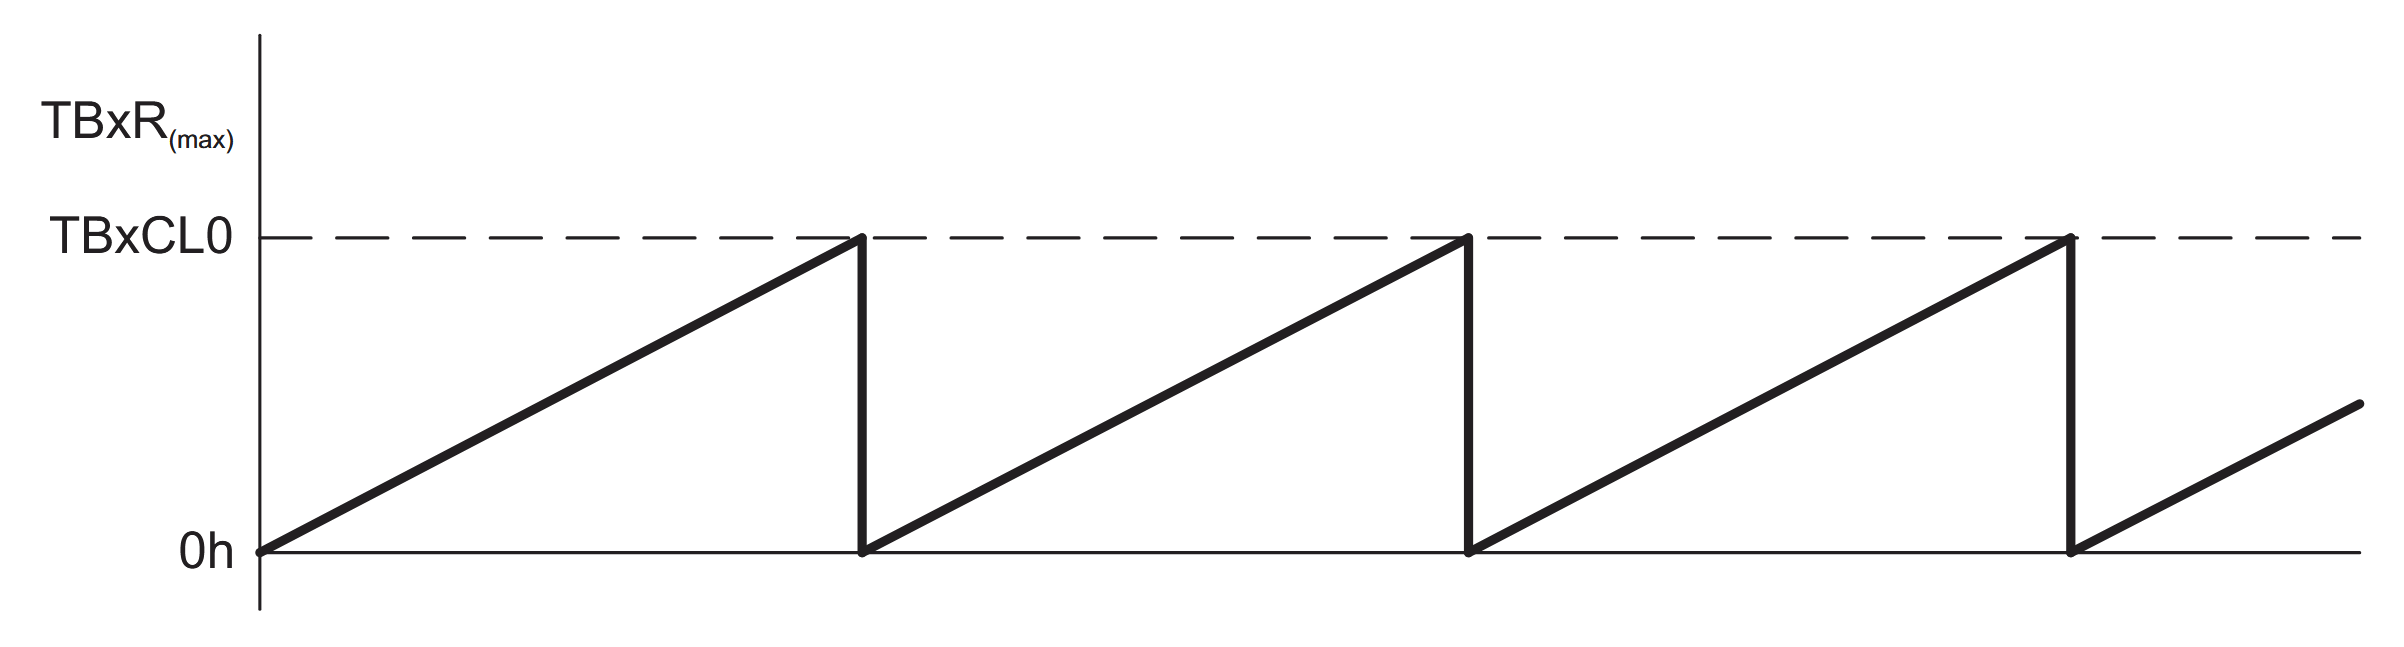
\includegraphics[width=0.75\textwidth]{../Bilder/up_mode.png}
		\caption{Up Mode \Zitat[S. 359, Abb. 12.2]{ti:slau272d}}
		\label{fig:up_mode}
	\end{figure}
	
	\item \textbf{Continuous Mode:} Der Continuous Mode (\Vgl \Abbildung{continuous_mode}) l\"asst den Z\"ahler von Null bis zum maximal m\"oglichen Wert (FFFFh f\"ur 16-Bit-Timer) z\"ahlen und anschlie{\ss}end wieder bei Null beginnen. Ein \"uberlauf-Interrupt wird generiert, wenn der Z\"ahler vom Wert von FFFFh auf 0 \"uberl\"auft. \Zitat[S. 338, Kap. 11.2.3.2 \& S. 360, Kap. 12.2.3.2]{ti:slau272d} Dieser Modus ist besonders n\"utzlich, wenn l\"angere, voneinander unabh\"angige Zeitintervalle zu messen sind oder eine freilaufende Zeitbasis ben\"otigt wird, um Ereignisse in Bezug auf den Z\"ahlerstand, ohne einen periodischen Neustart durch das Compare-Register, zu erfassen. \Zitat[S. 338, Kap. 11.2.3.3 \& S. 360, Kap. 12.2.3.3, S. 318, Kap. 8.5]{ti:slau272d, davies:msp430}
	
	\begin{figure}[h!]
		\centering
		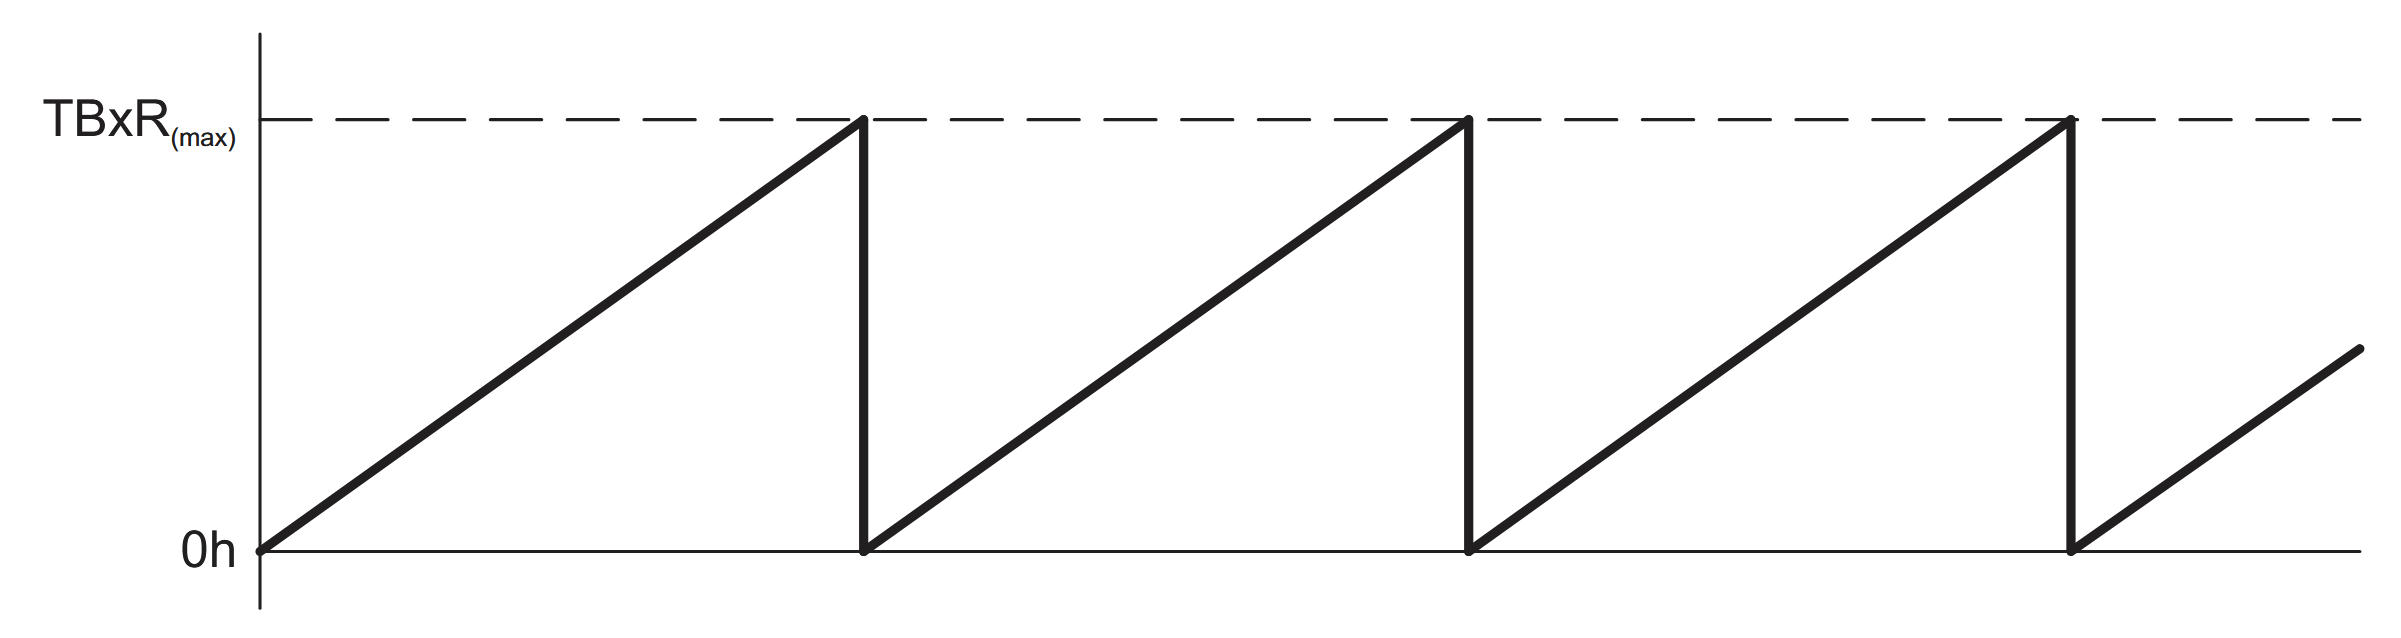
\includegraphics[width=0.75\textwidth]{../Bilder/continuous_mode.png}
		\caption{Continuous Mode \Zitat[S. 360, Abb. 12.4]{ti:slau272d}}
		\label{fig:continuous_mode}
	\end{figure}

	\item \textbf{Up/Down Mode:} Der Up/Down Mode (Auf-/Abw\"artsz\"ahlmodus, \Vgl \Abbildung{UpDown_mode}) kombiniert das Auf- und Abz\"ahlen. Der Z\"ahler beginnt bei Null, z\"ahlt Zyklisch bis zum festgelegten Wert im Compare-Register und dann wieder bis Null herunter. Ein \"uberlauf-Interrupt wird generiert, wenn der Z\"ahler den Wert von CCR0 erreicht, und ein weiterer Interrupt (sofern aktiviert) kann beim Erreichen von Null gesetzt werden. \Zitat[S. 339, Kap. 11.2.3.4 \& S. 361, Kap. 12.2.3.4]{ti:slau272d} Dieser Modus erzeugt eine symmetrische \Fachbegriff{Ein Verfahren zur Steuerung der Leistungszufuhr, bei dem die mittlere Ausgangsleistung durch Variieren des Abtastverh\"altnisses eines Rechtecksignals reguliert wird.}{Pulsweitenmodulation} (\Abkuerzung{Pulsweitenmodulation}{PWM}) und wird h\"aufig in Anwendungen zur Motorsteuerung oder zur Erzeugung pr\"aziser analoger Ausgangssignale eingesetzt. \Zitat[S. 340, Kap. 11.2.3.5 \& S. 362, Kap. 12.2.3.5, S. 349, Kap. 8.7]{ti:slau272d, davies:msp430}
	
	\begin{figure}[h!]
		\centering
		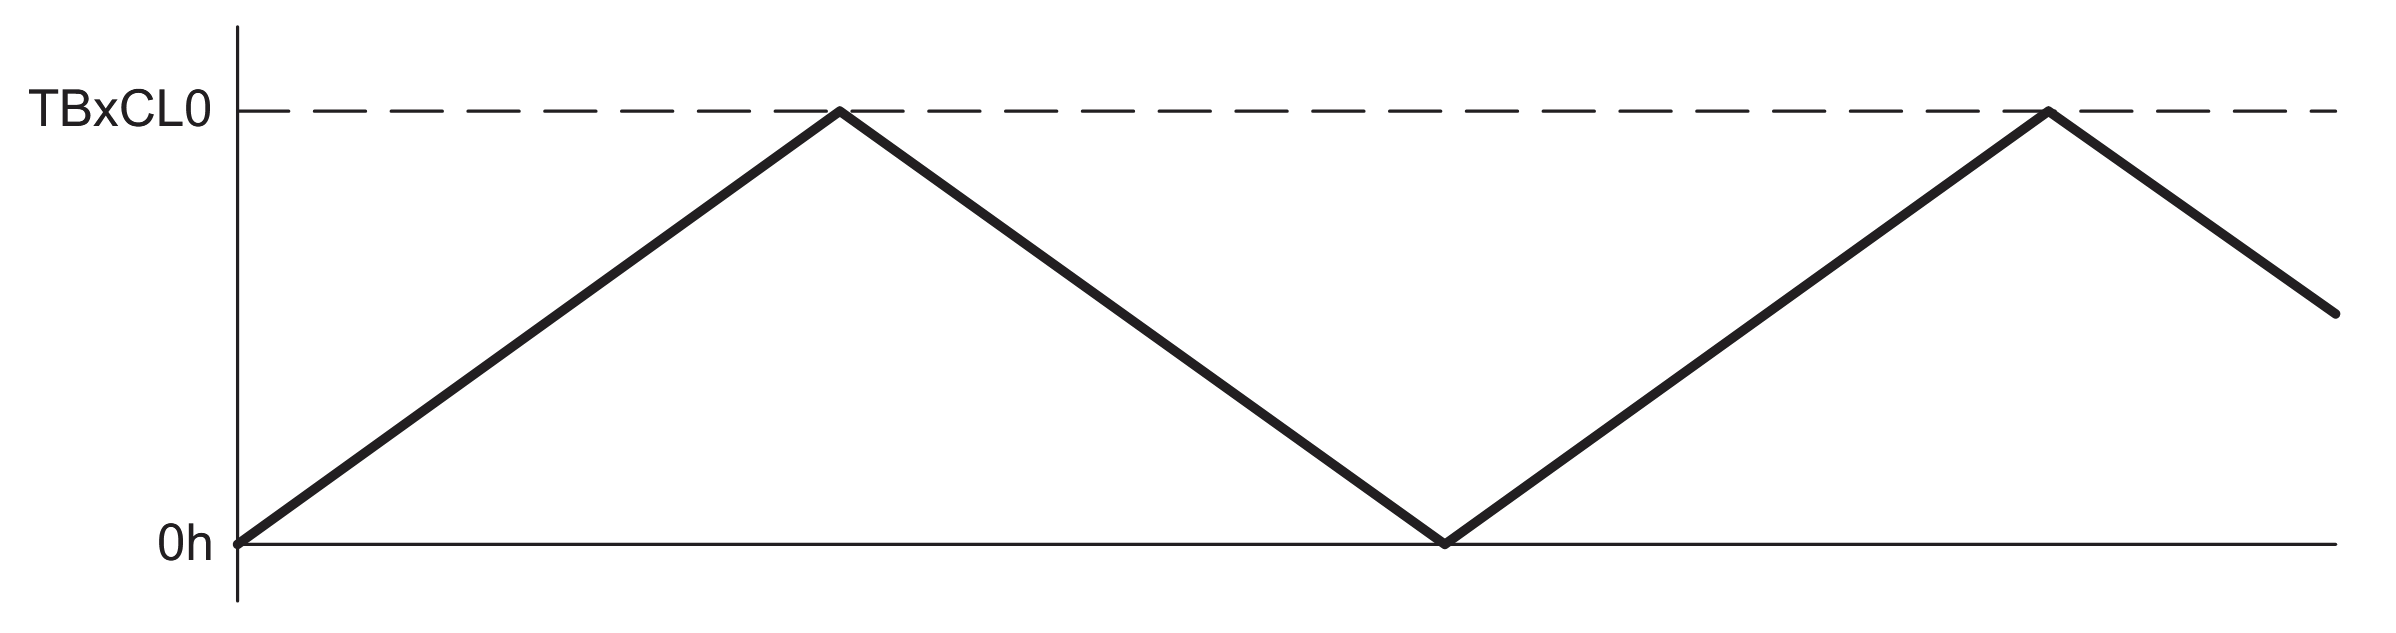
\includegraphics[width=0.75\textwidth]{../Bilder/up_down_mode.png}
		\caption{Up/Down Mode \Zitat[S. 361, Abb. 12.7]{ti:slau272d}}
		\label{fig:UpDown_mode}
	\end{figure}
\end{itemize}

Die Wahl eines geeigneten Modus h\"angt stark von der spezifischen Anwendung ab. F\"ur einfache Zeitmessungen oder periodische Aufgaben ist der Up Mode oft ausreichend, w\"ahrend der Continuous Mode f\"ur l\"angere Intervalle oder als Basis f\"ur komplexere Zeitsteuerungen dient. Der Up/Down Mode hingegen findet seine Anwendung prim\"ar in der Erzeugung von Steuersignalen.

Zur Erg\"anzug der drei Z\"ahlweisen des Timers, wird in den folgenden Kapiteln die genaue Rolle der bereits erw\"ahnten Capture-/Compare-Modi erläutert.

\newpage
\subsection{Capture-Mode}
\label{sec:Timer_CaptureMode}

Der Capture Mode erm\"oglicht es, den aktuellen Wert des Z\"ahlers pr\"azise zu erfassen, wenn ein bestimmtes Ereignis an einem zugeh\"origen Eingangspin auftritt. Der erfasste Z\"ahlerwert wird in einem der Capture-Register (\Code{CCR0} bis \Code{CCR6}) gespeichert. Dies ist besonders n\"utzlich f\"ur die Messung von externen Signalen wie Pulsweiten, Frequenzen oder der Zeit zwischen zwei Ereignissen. Beispiele hierzu in \Abbildung{CaptureModeBeispiele}.

\begin{figure}[h!]
	\centering
	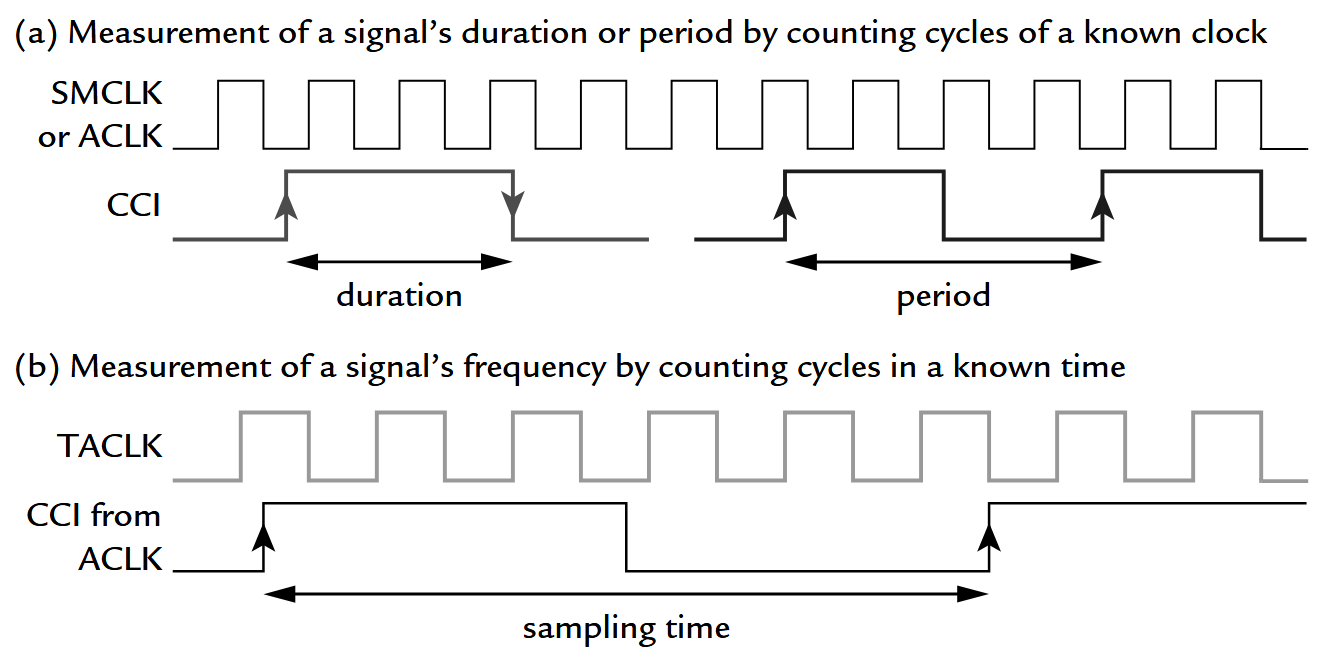
\includegraphics[width=1.0\textwidth]{../Bilder/CaptureMode_Beispiele.png}
	\caption{Capture Mode Einsatzbeispiele\\\Zitat[S. 301, Abb. 8.7]{davies:msp430}}
	\label{fig:CaptureModeBeispiele}
\end{figure}

Die Timer des MSP430FR5729 unterst\"utzen verschiedene Capture-Modi. Diese legen fest, bei welcher Art von Signal\"anderung die Erfassung des Z\"ahlerwertes erfolgt:

\begin{itemize}
	\item \textbf{Capture on rising edge:} Sobald am zugeh\"origen Eingangspin eine steigende Flanke detektiert wird (\"ubergang von Low nach High) wird in diesem Modus der aktuelle Z\"ahlerwert in das Capture-Register geschrieben.

	\item \textbf{Capture on falling edge:} Hier erfolgt die Erfassung des Z\"ahlerwertes am Eingangspin bei einer fallenden Flanke (\"ubergang von High nach Low).

	\item \textbf{Capture on both edges:} Dieser Modus erm\"oglicht die Erfassung des Z\"ahlerwertes sowohl bei steigender als auch fallender Flanken. Dies ist besonders praktisch f\"ur die Messung von Signalperioden oder bei Relevanz beider Flanken eines Signals.
\end{itemize}

Sofern ein Interrupt im entsprechenden Capture-Register aktiviert ist, kann dieser auch Interrupts ausl\"osen. In der zugeh\"origen ISR kann der erfasste Z\"ahlerwert aus dem Capture-Register gelesen und weiterverarbeitet werden. Mehrere Capture-Register innerhalb eines Timers erm\"oglichen die Erfassung und Auswertung mehrerer aufeinanderfolgender Ereignisse, ohne dass der vorherige Wert \"uberschrieben wird. 

Die Konfiguration des Capture Mode umfasst die Auswahl des ausl\"osenden Ereignisses (Flanke) sowie \ggf die Aktivierung des Capture-Interrupts. Die erfassten Zeitstempel im Capture-Register erlauben pr\"azise Messungen und die Analyse externer Signale in eingebetteten Systemen. \Zitat[S. 340, Kap. 11.2.4.1 \& S. 362, Kap. 12.2.4.1, S. 300, Kap. 8.4]{ti:slau272d, davies:msp430}

\subsection{Compare-Mode}
\label{sec:Timer_CompareMode}

Der Compare Mode erm\"oglicht es, den aktuellen Wert des Z\"ahlers kontinuierlich mit den in den Compare-Registern \Code{CCR0} bis \Code{CCR7} hinterlegten Werten zu vergleichen. Wenn der Z\"ahlerstand mit dem Vergleichswert \"ubereinstimmt, kann \zB ein Interrupt ausgel\"ost oder ein Ausgangspin beeinflusst werden.

Die Compare-Modi bieten verschiedene M\"oglichkeiten, wie der Ausgangspin bei einer \"ubereinstimmung beeinflusst werden soll:

\begin{itemize}
	\item \textbf{Set output on compare:} Bei einer \"ubereinstimmung des Z\"ahlerstandes mit dem Compare-Registerwert wird der zugeh\"orige Ausgangspin auf High gesetzt.

	\item \textbf{Reset output on compare:} Hier wird der Ausgangspin bei \"ubereinstimmung auf Low gesetzt.

	\item \textbf{Toggle output on compare:} In diesem Modus \"andert der Ausgangspin bei jeder \"ubereinstimmung seinen Zustand (von High nach Low oder von Low nach High).

	\item \textbf{Output High:} Der Ausgangspin wird permanent auf High gehalten.

	\item \textbf{Output Low:} Der Ausgangspin wird permanent auf Low gehalten.

	\item \textbf{Set/Reset:} In Kombination mit dem Compare-Register Null (\Code{CCR0}) kann ein PWM-Signal erzeugt werden. Beispielsweise kann der Ausgang bei Erreichen des \Code{CCR0}-Wertes gesetzt und bei Erreichen des \Code{CCRn}-Wertes zur\"uckgesetzt werden (oder umgekehrt), wobei \Code{CCRn} die Pulsweite bestimmt.
\end{itemize}

\Abbildung{OutputUnit_UpDown_Mode} zeigt eine m\"ogliche Konfiguration im Z\"ahlmodus Up/Down mit zwei Compare-Registern (\Code{TAxCCR1} \& \Code{TAxCCR2}), eingestellt auf Toggle/Set und Toggle/Reset.

\begin{figure}[h!]
	\centering
	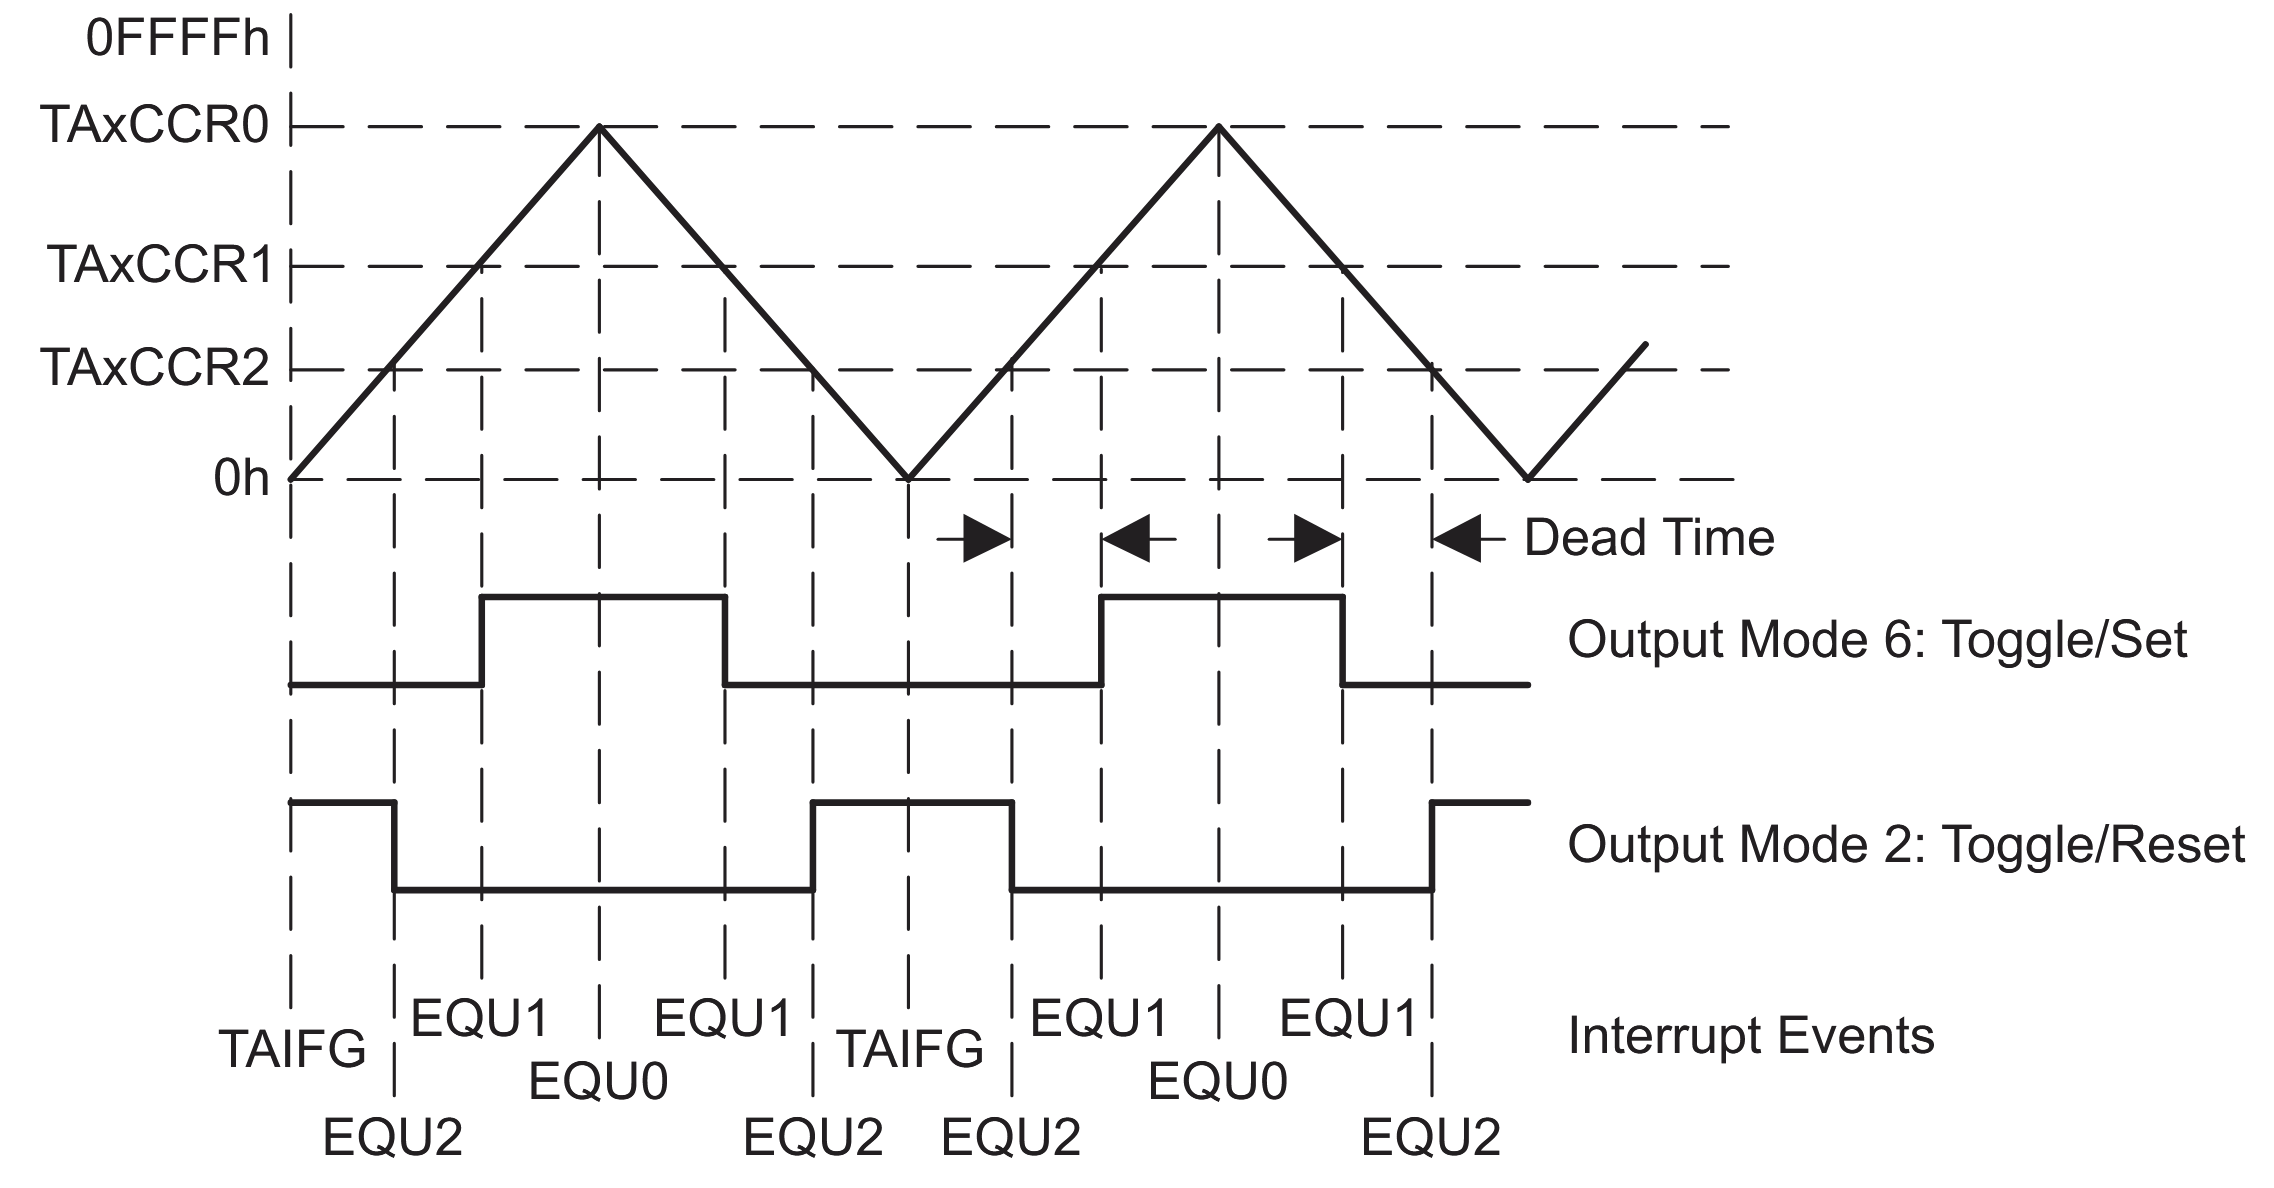
\includegraphics[width=1.0\textwidth]{../Bilder/UpDown_ModeBsp.png}
	\caption{Ausgabeeinheit im Up/Down-Modus\\\Zitat[S. 340, Abb. 11-9]{ti:slau272d}}
	\label{fig:OutputUnit_UpDown_Mode}
\end{figure}

\"Ahnlich wie beim Capture Mode erm\"oglicht ein Interrupt der CPU, auf pr\"azise Zeitpunkte zu reagieren und entsprechende Aktionen auszuf\"uhren. Der Compare Mode ist somit ein vielseitiges Werkzeug zur Erzeugung von Steuersignalen, zur Implementierung von Zeitverz\"ogerungen oder zur Synchronisation interner Operationen mit einer pr\"azisen Zeitbasis. \Zitat[S. 342, Kap. 11.2.4.2 \& S. 364, Kap. 12.2.4.2, S. 352, Kap. 8.8]{ti:slau272d, davies:msp430}

Nachdem die verschiedenen Betriebsarten des Timers betrachtet wurden, ist es wichtig zu verstehen, wie die zugeh\"origen Register konfiguriert werden, um die gew\"unschte Funktionalit\"at zu erzielen.

\newpage
\subsection{Einstellungen der Capture and Compare Register}
\label{sec:CC_Register}

Die Funktionalit\"at der Capture- und Compare-Einheiten wird ma{\ss}geblich durch die Konfiguration ihrer zugeh\"origen Register bestimmt. Hierzu geh\"oren die Aktivierung und Deaktivierung von Interrupts, die Auswahl des Ausgangsmodus (nur f\"ur Compare) sowie die Festlegung des ausl\"osenden Ereignisses.

F\"ur jedes Capture/Compare-Register kann individuell festgelegt werden, ob ein Interrupt ausgel\"ost werden soll, wenn ein entsprechendes Ereignis eintritt. Dies geschieht \"uber spezifische \NeuerBegriff{Interrupt-Enable-Bits} im jeweiligen Capture/Compare-Control-Register (\Code{TAxCCTLn} oder \Code{TBxCCTLn}). Beispielsweise durch das Setzen des \Code{CCIE}-Bits auf Eins oder Null, kann die Generierung eines Interrupts bei einem Capture- oder Compare-Ereignis aktiviert \bzw deaktiviert werden. \Tabelle{tb_ccc_register} fasst alle Register, beispielhaft anhand des Timers B, mit ihren Beschreibungen zusammen.


\begin{table}[h!]
	\small
	\centering
	\begin{tabular}{|c|l|c|c|p{8cm}|}
		\hline
		\textbf{Bit} & \textbf{Feld} & \textbf{Typ} & \textbf{Reset} & \textbf{Beschreibung} \\ \hline
		15-14 & CM & RW & 0h & Capture mode \\ \hline
		13-12 & CCIS & RW & 0h & Capture/compare input select. \"Uber diese Bits wird das \Code{TBxCCRn} Input-Signal ausgew\"ahlt. \\ \hline
		11 & SCS & RW & 0h & Synchronize capture source. Dieses Bit entscheidet, ob das Capture-Input-Signal mit der Timer-Clock synchronisiert wird. \\ \hline
		10-9 & CLLD & RW & 0h & Compare latch load. Ausw\"ahlen des \grqq compare latch load events\grqq. \\ \hline
		8 & CAP & RW & 0h & Capture-/Compare mode \\ \hline
		7-5 & OUTMOD & RW & 0h & Output mode \\ \hline
		4 & CCIE & RW & 0h & Capture/compare interrupt enable. Aktivieren der Interrupt-Anforderung des entsprechenden \Code{CCIFG}-Flag. \\ \hline
		3 & CCI & R & Undef & Capture/compare input. Das ausgew\"ahlte Eingangssignal kann \"uber dieses Bit ausgelesen werden. \\ \hline
		2 & OUT & RW & 0h & Output. F\"ur Output-Mode \grq 0\grq{} kontrolliert dieses Bit den Ausgangsstatus. \\ \hline
		1 & COV & RW & 0h & Capture overflow. Dieses Bit zeigt ein \grqq capture overflow\grqq an. \Code{COV} muss Softwareseitig zur\"uckgesetzt werden.  \\ \hline
		0 & CCIFG & RW & 0h & Capture/compare interrupt flag \\ \hline
	\end{tabular}
	\caption{Registerbeschreibung – Capture-/Compare Register Timer B \\ \Zitat[S. 375, Tab. 12-8]{ti:slau272d}}
	\label{tab:tb_ccc_register}
\end{table}

\newpage
Wie bereits in \Kapitel{Timer_CompareMode} zum Compare-Modus beschrieben, legen die Output-Mode-Bits (\Code{OUTMOD}) fest, wie der zugeh\"orige Ausgangspin bei einer \"ubereinstimmung des Z\"ahlerstandes mit dem Compare-Registerwert beeinflusst wird. Die Auswahl des passenden Output-Modus ist entscheidend f\"ur die Erzeugung der gew\"unschten Ausgangssignale, wie beispielsweise bei der Pulsweitenmodulation.

Die Auswahl des ausl\"osenden Ereignisses f\"ur eine Capture- oder Compare-Operation wird ebenfalls \"uber Bits im \Code{TAxCCTLn}- oder \Code{TBxCCTLn}-Register gesteuert. F\"ur den Capture-Modus wird hier beispielsweise mit dem \Code{CM}-Bit festgelegt, ob die Erfassung bei einer steigenden, fallenden oder bei beiden Flanken des Eingangssignals erfolgen soll. Im Compare-Modus definiert diese Einstellung, unter welchen Bedingungen die Vergleichsoperation als erfolgreich betrachtet wird und die entsprechende Aktion (Interrupt, Ausgangssignal\"anderung) ausgel\"ost wird. Dies kann beispielsweise ein reiner Vergleich oder auch ein Vergleich in Kombination mit dem \"uberlauf des Z\"ahlers im Up-Modus sein. \Zitat[S. 351, Kap. 11.3.3 \& S. 375, Kap. 12.3.3, S. 292, Kap. 8.3.2]{ti:slau272d, davies:msp430}

Die sorgf\"altige Konfiguration dieser Einstellungen in den Capture/Compare-Registern ist unerl\"asslich, um den Timer an die Anforderungen der jeweiligen Applikation anzupassen.

Ein weiterer fundamentaler Aspekt der Timer-Konfiguration ist \ua die Wahl der Taktquelle, welche die Zeitbasis f\"ur den Z\"ahler und somit f\"ur alle zeitgesteuerten Operationen des Timers bestimmt.\AI

\newpage
\subsection{Timer Control-Register}
\label{sec:TimerControlRegister}

Die Timer des MSP430FR5729 k\"onnen von verschiedenen internen Taktquellen getaktet werden, die jeweils unterschiedliche Eigenschaften und Anwendungsbereiche aufweisen. Die prim\"aren Taktquellen sind \Fachbegriff{Niederfrequente Taktquelle in Mikrocontroller-Systemen, die typischerweise von einem Quarzoszillator gespeist wird und f\"ur energiesparende Betriebsmodi verwendet wird.}{Auxiliary Clock} (\Abkuerzung{Auxiliary Clock}{ACLK}) und \Fachbegriff{Taktgesteuertes Signal, das typischerweise f\"ur Peripherieger\"ate verwendet wird und sich aus einer frei w\"ahlbaren Taktquelle ableiten l\"asst.}{Sub-Main Clock} (\Abkuerzung{Sub-Main Clock}{SMCLK}). Auch externe Taktquellen k\"onnen zur Taktung des Timers herangezogen werden wie \zB das \Code{TACLK}/\Code{TBCLK}-Register oder der \Code{INCLK}-Pin. \\\Zitat[S. 71, Kap. 3.1, S. 163, Kap. 5.8 \& S. 289, Kap. 8.3.1]{ti:slau272d, davies:msp430}

Die Auswahl einer geeigneten \glqq Clock-Source\grqq{} f\"ur den Timer erfolgt \"uber spezifische Bits im \Code{TAxCTL} oder \Code{TBxCTL} Timer-Control-Register. Das \Code{TASSEL}-/\Code{TBSSEL}-Bit legt fest, ob der Timer von \Code{TAxCLK}/\Code{TBxCLK}, \Code{ACLK}, \Code{SMCLK} oder \Code{INCLK} getaktet wird. Diese Wahl hat einen direkten Einfluss auf die Timer-Frequenz, wobei sie nicht gleich der Frequenz der gew\"ahlten Clock-Source entsprechen muss. Durch optionale \Fachbegriff{Vorschaltglied in elektronischen Z\"ahlschaltungen oder Timern, welches die Frequenz eines Eingangssignals durch einen festen Faktor reduziert, um eine nachfolgende Verarbeitung mit geringerer Taktrate zu erm\"oglichen.}{Prescaler-Werte}[Prescaler] wie dem \Code{ID}-Bit und dem \Code{TAIDEX}-/\Code{TBIDEX}-Bit kann die Frequenz weiter individualisiert werden. \Zitat[S. 349, Kap. 11.3.1 \& S. 372, Kap. 12.3.1, S. 289, Kap. 8.3.1]{ti:slau272d, davies:msp430}

Die Timer-Frequenz bestimmt wiederum die Zeitbasis des Timers. Eine h\"ohere Timer-Frequenz f\"uhrt zu einer feineren Zeitaufl\"osung, da der Z\"ahler schneller inkrementiert wird. Dies erm\"oglicht pr\"azise Zeitmessungen und die Erzeugung von Signalen hoher Frequenzen. Umgekehrt f\"uhrt eine niedrigere Frequenz zu einer gr\"oberen Zeitaufl\"osung, kann aber den Stromverbrauch reduzieren.

Ein weiteres Steuerbit, das \glqq Mode Control\grqq{}-Bit (\Abkuerzung{Mode Control}{\Code{MC}}) steuert die -- bereits in \Kapitel{Timer_CountMode} erl\"auterten -- Z\"ahl-Modi und das \Code{TAIE}-/\Code{TBIE}-Bit steuert, ob Interrupts Ein- oder Ausgeschaltet sind.

Die Auswahl der Clock-Source, des Prescalers und weiteren Steuerbits ist daher entscheidend, um die gew\"unschte Zeitbasis, Aufl\"osung und Verhalten f\"ur den zu konfigurierenden Timer zu erreichen um die Anforderungen der jeweiligen Anwendung optimal zu erf\"ullen.

\newpage
\Tabelle{tb_c_register} fasst alle weiteren Register des Timers B mit ihren Beschreibungen zusammen.\AI

\begin{table}[h!]
	\small
	\centering
	\begin{tabular}{|c|l|c|c|p{8cm}|}
		\hline
		\textbf{Bit} & \textbf{Feld} & \textbf{Typ} & \textbf{Reset} & \textbf{Beschreibung} \\ \hline
		15 & Reserved & R & 0h & Reserved. Immer als 0 gelesen. \\ \hline
		14–13 & TBCLGRP & RW & 0h & \textbf{\Code{TBxCLn}-group;} Synchrone Aktualisierung mehrerer Capture/Compare-Register. \\ \hline
		12–11 & CNTL & RW & 0h & Counter length \\ \hline
		10 & Reserved & R & 0h & Reserved. Immer als 0 gelesen. \\ \hline
		9–8 & TBSSEL & RW & 0h & clock source select \\ \hline
		7–6 & ID & RW & 0h & \textbf{Input divider;} Teilung der gew\"ahlten Clock-Source in Verbindung mit dem \Code{TBIDEX}-Register. \\ \hline
		5–4 & MC & RW & 0h & \textbf{Mode control;} Ausf\"uhrlicher in \Kapitel{Timer_CountMode} \\ \hline
		3 & Reserved & R & 0h & Reserved. Immer als 0 gelesen. \\ \hline
		2 & TBCLR & RW & 0h & Setzt \Code{TBR} und Kontroll-Logik zur\"uck. \\ \hline
		1 & TBIE & RW & 0h & Timer\_B interrupt enable \\ \hline
		0 & TBIFG & RW & 0h & Timer\_B interrupt flag \\ \hline
	\end{tabular}
	\caption{Registerbeschreibung – Control Register Timer B\\\Zitat[S. 372, Tab. 12-6]{ti:slau272d}}
	\label{tab:tb_c_register}
\end{table}

\subsection{Zusammenfassung und Einsatzm\"oglichkeiten}
\label{sec:TimerEinsatzmoeglichkeiten}

Die detaillierte Auseinandersetzung mit der Timer-Architektur des MSP430FR5729 hat die Flexibilit\"at und Leistungsf\"ahigkeit dieser Peripheriekomponente verdeutlicht. Die Unterscheidung zwischen Timer des Typs A und B, die verschiedenen Betriebsarten (Z\"ahlmodus und Capture/Compare) sowie die vielf\"altigen Einstellm\"oglichkeiten der Steuerregister und die Auswahl der Taktquelle er\"offnen ein breites Spektrum an Anwendungsm\"oglichkeiten in eingebetteter Software.

Analog zur \"Ubersicht \glqq What Timer Where?\grqq{} von John H. Davies lassen sich die prim\"aren Einsatzgebiete der Timer des MSP430FR5729 wie folgt zusammenfassen: \Zitat[S. 356, Kap. 8.10]{davies:msp430}

\newpage
\begin{itemize}
	\item \textbf{Zeitmessung und Zeitbasis:} Unabh\"angig vom Timer-Typ k\"onnen alle als eine pr\"azise Zeitbasis dienen. Durch die Wahl einer geeigneten Clock-Source und passender Prescaler-Werte lassen sich genaue Zeitintervalle festlegen. Dies ist fundamental f\"ur das Zeitmanagement innerhalb des Mikrocontrollers und die Synchronisation mit externen als auch Internen Ereignissen. Timer A eignet sich hierbei oft f\"ur grundlegende Zeitsteuerungsaufgaben, w\"ahrend die flexiblere Konfigurierbarkeit des Timers vom Typ B wie \zB verschiedene Bit-L\"angen (\Kapitel{TIMER&ISR}) eine feinere Anpassung an spezifische Zeitmessanforderungen erlaubt.

	\item \textbf{Ereigniserfassung (Capture):} Die Capture-Funktionalit\"at erm\"oglicht eine pr\"azise Erfassung des Zeitpunkts externer -- oder \ggf auch interner -- Ereignisse. Dies ist unerl\"asslich f\"ur Anwendungen wie die Messung von Pulsweiten, die Frequenzmessung von Signalen oder die Erfassung der Ankunftszeit von Informationen in Kommunikationsprotokollen. Die M\"oglichkeit, sowohl steigende, fallende Flanken oder auch beide zu erfassen, erweitert den Anwendungsbereich in vielen verschiedenen Szenarien.

	\item \textbf{Signalerzeugung (Compare/PWM):} Die Compare-Einheiten in Verbindung mit den verschiedenen Ausgangsmodi erlauben die Generierung pr\"aziser Ausgangssignale. Dies ist besonders relevant f\"ur die Pulsweitenmodulation, die zur Steuerung von Motoren, zur Dimmung von LEDs oder zur Erzeugung analog wirkender Signale eingesetzt wird. Der Up/Down Mode des Count-Modus in Kombination mit den Compare-Registern des Timer B bietet hierbei besonders flexible M\"oglichkeiten zur Erzeugung verschiedenster PWM-Signale.

	\item \textbf{Interrupt-Steuerung und Task-Rotation:} Sowohl Capture- als auch Compare-Ereignisse k\"onnen Interrupts ausl\"osen. Dies erm\"oglicht eine effiziente Reaktion des Mikrocontrollers auf zeitgesteuerte Ereignisse oder Signale, ohne die kontinuierliche abfrage des Timer-Status. Die pr\"azise Interrupt-Generierung tr\"agt ma{\ss}geblich zur Realisierung reaktiver und effizienter eingebetteter (Echtzeit-) Systeme bei.
\end{itemize}

\newpage
Zusammenfassend l\"asst sich der grundlegende Aufbau eines Timers, vereinfacht nach dem Vorbild aus Abbildung 8.5 und Abbildung 8.16 aus Davies' Buch, wie folgt darstellen:

Ein Timer besteht im Kern aus einem Z\"ahler (\Kapitel{Timer_CountMode}), der durch eine ausgew\"ahlte Clock-Source (\Kapitel{TimerControlRegister}) in definierten Schritten inkrementiert oder dekrementiert wird. Dieser Z\"ahler l\"auft gem\"a{\ss} der gew\"ahlten Betriebsart.

Zus\"atzlich verf\"ugt der Timer \"uber Sieben Capture/Compare-Kan\"ale. Jeder Kanal beinhaltet mindestens ein Capture/Compare-Register sowie die zugeh\"orige Steuereinheit.

Im Capture Mode (\Kapitel{Timer_CaptureMode}) wird der aktuelle Wert des Z\"ahlers in das \Code{CCRx}-Register geschrieben, wenn ein durch die Steuereinheit ausgew\"ahltes Ereignis (\zB Flanke an einem Eingangspin) eintritt.

Im Compare Mode (\Kapitel{Timer_CompareMode}) wird der aktuelle Wert des Z\"ahlers kontinuierlich mit dem Wert im \Code{CCRx}-Register verglichen. Bei einer \"Ubereinstimmung l\"ost die Steuereinheit eine konfigurierte Aktion aus, wie beispielsweise das Setzen/R\"ucksetzen/Toggeln eines zugeh\"origen Ausgangspins oder die Generierung eines Interrupts, sofern dieser in der Steuereinheit aktiviert wurde.

Die Steuereinheit erm\"oglicht die Konfiguration des jeweiligen Kanals, einschlie{\ss}lich der Auswahl des Capture/Compare-Modus, des ausl\"osenden Ereignisses, des Ausgangsmodus und der Aktivierung/Deaktivierung des Interrupts.

\newpage
Das Blockdiagramm in \Abbildung{BlockDiagramm_Timer} zeigt Timer B mit seinen grundlegenden Komponenten und deren Zusammenspiel. Die flexiblen Konfigurationsm\"oglichkeiten dieser Bl\"ocke erm\"oglicht die Realisierung einer Vielzahl von Zeitsteuerungs- und Signalverarbeitungsaufgaben.

\begin{figure}[h!]
	\centering
	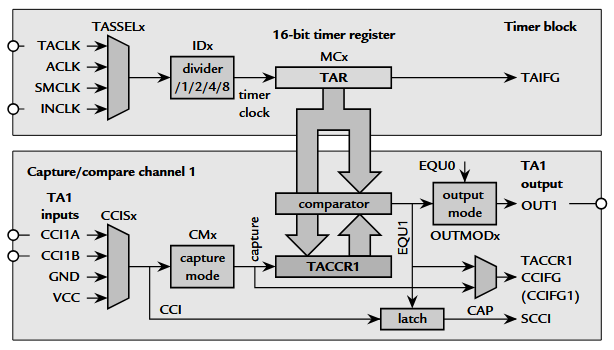
\includegraphics[width=1.0\textwidth]{../Bilder/BlockDiagram_TimerB.png}
	\caption{Timer B Block \& Capture/Compare Channel 1\\\Zitat[S. 355, Kap. 8.16]{davies:msp430}}
	\label{fig:BlockDiagramm_Timer}
\end{figure}

\newpage
\section{Enhanced Universal Serial Communication Interface (eUSCI)}
\label{sec:eUSCI}

Das eUSCI ist eine vielseitige und flexible serielle Peripheriekomponente des MSP430FR5729. Sie erm\"oglicht die Kommunikation mit externen Ger\"aten und Systemen \"uber zahlreiche Schnittstellen und Protokolle. Auch Sensoren, Aktoren und Speichermedien werden \"uber diese weise mit dem System verbunden. Dieses Kapitel beleuchtet die Architektur des \Fachbegriff{Ein Interface bezeichnet in der Informatik eine definierte Schnittstelle, \"uber die Komponenten eines Softwaresystems miteinander kommunizieren k\"onnen, ohne deren interne Implementierung zu kennen.}{Interfaces}[Interface], seine verschiedenen Betriebsmodi und Konfigurationsm\"oglichkeiten bereitgestellter Kommunikationstechnologien.

Der MSP430FR5729 verf\"ugt \"uber zwei Kommunikationskan\"ale, die in den folgenden Kapiteln n\"aher betrachtet werden. 

\subsection{Die eUSCI-Architektur}
\label{sec:eUSCI_Architektur}

Jede Form der \Fachbegriff{Die \"Ubertragung von Datenbitfolgen \"uber eine einzelne Leitung, wobei die Bits nacheinander (also \glqq seriell\grqq{}) gesendet werden. Sie wird h\"aufig bei einfachen oder ressourcenschonenden Datenverbindungen eingesetzt, \zB \"uber UART, SPI oder I$^{2}$C.}{Seriellen Kommunikation}[Serielle Kommunikation] basiert auf einem Taktgeber. Der zentrale Unterschied zwischen Protokollen liegt im Timing: Wann gestattet der Taktgeber dem Sender das Schreiben des n\"achsten Bits auf einen Ausgangskanal und dem Empf\"anger das Lesen des kommenden Bits. Dabei gibt es Synchrone und Asynchrone Ans\"atze, weshalb zwei Kommunikationskan\"ale bereitgestellt werden. \Zitat[S. 494, Kap. 10]{davies:msp430}

Beim MSP430FR5729 ist der Kommunikationskanal vom Typ-B f\"ur Synchrone Daten\"ubertragung optimiert, w\"ahrend Kanal A vorrangig f\"ur asynchrone \"Ubertragungsverfahren vorgesehen ist. \Zitat[S. 496, Kap. 10.1.2]{davies:msp430}

Der wesentliche Unterschied zwischen diesen beiden \"Ubertragungsarten besteht darin, ob das Taktsignal ebenfalls mit \"ubertragen wird. Bei der synchronen Kommunikation, wie sie etwa mit den Protokollen SPI oder I$^{2}$C erfolgt, wird dieses Taktsignal explizit mitgef\"uhrt. Im Gegensatz dazu kommt das UART-Protokoll ohne ein separates Taktsignal aus, da Sender und Empf\"anger \"uber eine gemeinsame Baudrate synchronisiert sind. \Zitat[S. 494, Kap. 10]{davies:msp430}

\newpage
Entsprechend ist der universelle Kommunikationskanal vom Typ B (\Abkuerzung{enhanced Universal Serial Communication Interface Type B}{eUSCI\_B}) speziell auf die Anforderungen synchroner Protokolle wie SPI und I$^{2}$C ausgelegt. Das \Abkuerzung{enhanced Universal Serial Communication Interface Type A}{eUSCI\_A}{}-Modul hingegen unterst\"utzt prim\"ar die UART-Kommunikation, kann jedoch dar\"uber hinaus auch eine asynchrone Variante des SPI-Protokolls abbilden. \Zitat[S. 496, Kap. 10.1.2]{davies:msp430}

\begin{table}[h!]
	\small
	\centering
	\begin{tabular}{|l|c|c|}
		\hline
		\textbf{Funktion} & \textbf{eUSCI\_A} & \textbf{eUSCI\_B} \\\hline
		UART (asynchron) & \checkmark & -- \\\hline
		SPI (synchron) & \checkmark (Master/Slave) & \checkmark (Master/Slave) \\\hline
		SPI (asynchron, nur TX) & \checkmark & -- \\\hline
		I\textsuperscript{2}C (synchron) & -- & \checkmark (Master/Slave) \\\hline
		LIN-kompatibel & \checkmark & -- \\\hline
		Automatische Baudratenerkennung (UART) & \checkmark & -- \\\hline
		Adress- und Broadcast-Modus (I\textsuperscript{2}C) & -- & \checkmark \\\hline
		Multimaster-Unterst\"utzung (I\textsuperscript{2}C) & -- & \checkmark \\\hline
	\end{tabular}
	\caption{Funktionsvergleich der eUSCI-Module des MSP430FR5729\\\Zitat[Kap. 18, 19, 20, S. 493, Kap. 10]{ti:slau272d, davies:msp430}}
	\label{tab:eusci-vergleich}
\end{table}

\Tabelle{eusci-vergleich} fasst nochmals alle Eigenschaften beider Kan\"ale zusammen und stellt sie gegen\"uber. Wobei Tiefgreifenderep protokollspezifische Funktionen in den entsprechenden Unterkapiteln n\"aher betrachtet werden.

\subsection{Einordnung vorhandener Kommunikationsschnittstellen}
\label{sec:Einordnung_Schnittstellen}

Die vorliegende Arbeit befasst sich mit der Entwicklung einer interruptgesteuerten Benutzerschnittstelle. Die Evaluation einer daf\"ur geeigneten Schnittstelle zur Interaktion mit externen \Abkuerzung{Personal Computer}{PC} Systemen bestimmt ma{\ss}geblich den weiteren Verlauf der Evaluation und des Projekts. Daher ist eine einf\"uhrende Einordnung der zur Verf\"ugung stehenden seriellen Protokolle erforderlich, um im weiteren Verlauf gezielt auf jene Technologie eingehen zu k\"onnen, die im Kontext der Arbeit von praktischer Relevanz ist.

Die Kommunikation \"uber synchrone Protokolle wie I$^{2}$C und SPI eignen sich besonders gut f\"ur den Datenaustausch zwischen einem Microcontroller und seinen Peripherieger\"aten oder weiteren Mikrocontrollern im Master-Slave-Verh\"altnis. Welche der beiden Technologien im jeweiligen Anwendungsfall zum Einsatz kommt, h\"angt unter anderem von der Anzahl der beteiligten Ger\"ate sowie der Distanz zu den Kommunikationspartnern ab. Weitere technische Unterschiede dieser Protokolle sind in \Tabelle{synchrone_protokolle} aufgelistet.

Zusammenfassend l\"asst sich feststellen, dass sich die synchrone Daten\"ubertragung nur bedingt f\"ur die Kommunikation mit einem auf Windows oder Linux basierenden System eignet. Im Gegensatz dazu sind asynchrone Protokolle wie UART f\"ur diese Art der Anwendung deutlich besser geeignet. 

Das UART-Protokoll zeichnet sich nicht nur durch eine einfache Implementierung aus, sondern ist auch \"au{\ss}erst robust und ressourcenschonend -- Eigenschaften, die insbesondere bei modularen, \Fachbegriff{Automatische Erkennung und Integration von Komponenten in ein System ohne manuelle Konfiguration}{Plug-and-Play-f\"ahigen}[Plug-and-Play] Systemkomponenten entscheidend sind. Der Verzicht auf eine gemeinsame Taktleitung erlaubt eine Punkt-zu-Punkt-Verbindung mit vergleichsweise geringen Hardwareanforderungen. 

Diese Vorteile gelten gleicherma{\ss}en f\"ur die gegen\"uberliegende Seite der Schnittstelle: Alle g\"angigen Betriebssysteme wie Windows, Linux oder macOS stellen standardm\"a{\ss}ig Treiber f\"ur die asynchrone serielle Daten\"ubertragung bereit. Unter Windows erfolgt dies beispielsweise \"uber sogenannte \NeuerBegriff{COM-Ports}, w\"ahrend unter Linux Schnittstellen wie \NeuerBegriff{/dev/ttySx} oder \NeuerBegriff{/dev/ttyUSBx} verwendet werden.

\newpage
\begin{table}[h!]
	\small
	\centering
	\begin{tabular}{|p{4.5cm}|p{4.5cm}|p{4.5cm}|}
		\hline
		\textbf{Kriterium} & \textbf{SPI} & \textbf{I$^{2}$C} \\\hline
		\textbf{Signalleitungen} & 4 Leitungen: SCLK, MOSI, MISO, CS (pro Slave) & 2 Leitungen: SCL (Takt), SDA (Daten) \\\hline
		\textbf{Adressierung} & Keine; Slaves \"uber eigene Chip Selects (CS) & Ja; \"uber 7- oder 10-Bit-Adresse auf dem Bus \\\hline
		\textbf{Daten\"ubertragung} & \Fachbegriff{Gleichzeitige Daten\"ubertragung in beide Richtungen}{Vollduplex} m\"oglich & \Fachbegriff{Daten\"ubertragung zu einem Zeitpunkt nur in eine Richtung m\"oglich}{Halbduplex} \\\hline
		\textbf{Taktfrequenz} & Bis > 10,MHz (ger\"ateabh\"angig) & Typisch 100,kHz, 400,kHz, bis 3.4,MHz (High-Speed) \\\hline
		\textbf{Komplexit\"at des Protokolls} & Einfach, ohne Start-/Stopp- oder ACK-Signale & H\"oher, mit Start-/Stoppbedingungen und Acknowledgements \\\hline
		\textbf{Multimaster-Unterst\"utzung} & Nein (standardm\"a{\ss}ig) & Ja \\\hline
		\textbf{Skalierbarkeit (Anzahl Ger\"ate)} & Eingeschr\"ankt, abh\"angig von verf\"ugbaren CS-Leitungen & Hoch, bis zu 128 Ger\"ate durch Adressierung \\\hline
		\textbf{Typische Einsatzgebiete} & Hochgeschwindigkeits-kommunikation (\zB SD-Karten, Displays) & Niedriggeschwindigkeits-Komponenten (\zB Sensoren, EEPROMs) \\\hline
		\textbf{Leitungsl\"ange / St\"oranf\"alligkeit} & Gut f\"ur kurze, direkte Verbindungen & H\"ohere Anf\"alligkeit f\"ur St\"orungen und Begrenzung durch Leitungskapazit\"at \\\hline
	\end{tabular}
	\caption{Vergleich der synchronen seriellen Protokolle SPI und I$^{2}$C\\\Zitat[S. 497, Kap. 10.2, S. 534, Kap. 10.7]{davies:msp430}}
	\label{tab:synchrone_protokolle}
\end{table}

Im Falle des MSP430FR5729 erfolgt die UART-Kommunikation zus\"atzlich interruptgesteuert. Dies erlaubt es, eingehende Daten \"uber eine eigens definierte ISR zu verarbeiten, was eine latenzarme, gleichzeitig jedoch energieeffiziente Verarbeitung erm\"oglicht.\Zitat[S. 574, Kap. 10.12]{davies:msp430}

Aus diesen Gr\"unden stellt UART die technisch sinnvollste Wahl f\"ur die Kommunikation zwischen dem MSP430FR5729 und einem PC mit Windows, Linux oder macOS dar. Das Protokoll erlaubt eine minimalinvasive, betriebssystemkompatible und energieeffiziente Verbindung. Im weiteren Verlauf wird die asynchrone universelle serielle Schnittstelle mit dem UART Protokoll detaillierter betrachtet.\AI

\subsection{eUSCI\_A Modul: UART-Modus (Asynchrone Kommunikation)}
\label{sec:eUSCI_UART}

F\"ur ein tiefgreifendes Verst\"andnis des Zusammenspiels zwischen dem Interface und dem UART-Protokoll ist es unerl\"asslich, zun\"achst die fundamentalen technischen Aspekte, notwendige Register und charakteristische Merkmale zu erl\"autern.

\subsubsection{Informations\"ubertragung}
\label{sec:UART_uebertragung}

Die Baudrate, wie in \Kapitel{eUSCI_Architektur} bereits er\"ortert, fungiert als entscheidender Synchronisationsmechanismus f\"ur asynchrone Daten\"ubertragungen. Dies impliziert, dass Sender und Empf\"anger sich zwar nicht an ein pr\"azises Timing f\"ur die \"Ubertragung einzelner Bits halten m\"ussen, jedoch eine \"Ubereinstimmung hinsichtlich der Frequenz zur \"Ubertragung ganzer Bl\"ocke -- typischerweise Bytes oder Zeichen -- erforderlich ist. \Abbildung{uart_send} visualisiert beispielhaft die \"Ubertragung zweier Bl\"ocke, die jeweils durch ein Start-Bit (\Abkuerzung{Start-Bit}{ST}) eingeleitet und durch ein Stop-Bit (\Abkuerzung{Stop-Bit}{SP}) abgeschlossen werden. Durch die Verwendung dieser Rahmenbits ergibt sich bei einer Konfiguration von acht Datenbits eine Netto-Datenrate von 8/10 der Brutto-\"Ubertragungsrate. Das bedeutet, dass von zehn \"ubertragenen Bits acht Bits die eigentliche Nutzinformation darstellt. Es gibt auch die M\"oglichkeit, flexibel auf unterschiedliche Baudraten zu reagieren. \"Uber die Automatische Baudraten-Erkennung, erl\"autert in \Kapitel{auto_baud}, kann mit mehreren Kommunikationspartnern unterschiedlicher Baudraten kommuniziert werden.

\begin{figure}[h!]
	\centering
	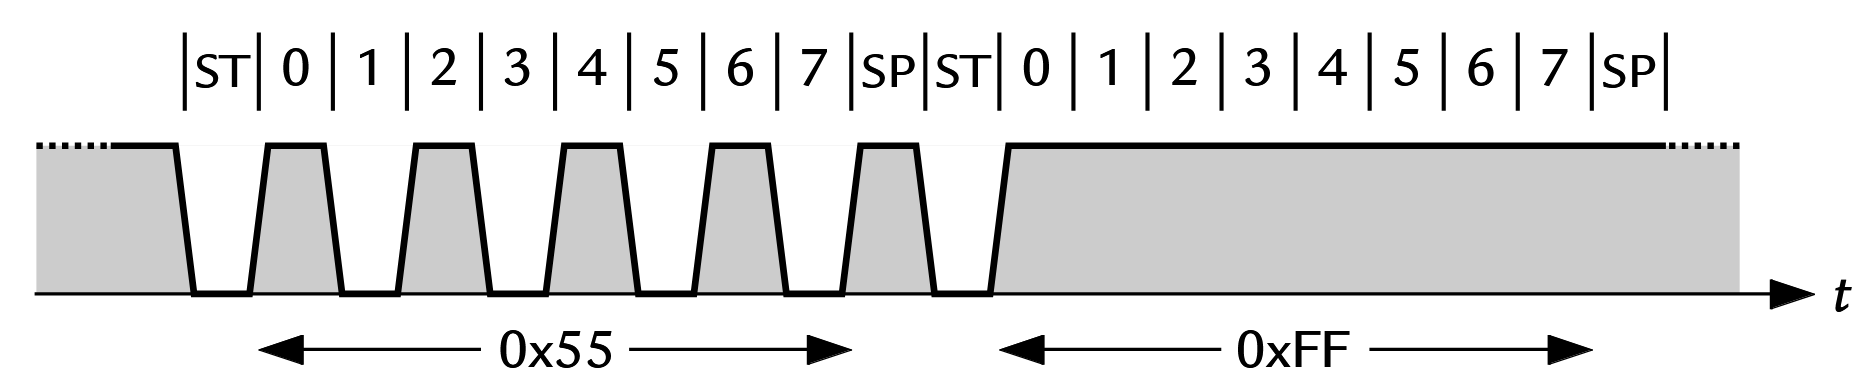
\includegraphics[width=1.0\textwidth]{../Bilder/Baudrate.png}
	\caption{UART \"ubertragung der Werte 0x55 und 0xFF\\\Zitat[S. 576, Abb. 10.18]{davies:msp430}}
	\label{fig:uart_send}
\end{figure}

\newpage
Die einzelnen Bits innerhalb eines Datenblocks werden mittels des \Fachbegriff{Bin\"ares Leitungscodierungsverfahren, bei dem der Signalpegel w\"ahrend eines Bitintervalls konstant bleibt und nicht zwischen den Bits auf einen Nullpegel zur\"uckkehrt}{Non-Return-to-Zero} (\Abkuerzung{non-return to zero}{NRZ})-Verfahrens kodiert und \"ubertragen. Eine typische Baudrate f\"ur eingebettete Systeme betr\"agt 9600 Baud, obgleich auch h\"ohere Frequenzen zur beschleunigten Daten\"ubertragung Anwendung finden k\"onnen.

Die physikalische Verbindung zweier Parteien wird \"ublicherweise \"uber drei Leitungen realisiert. Eine Leitung f\"ur jede Kommunikationsrichtung (\Abkuerzung{Transmit Data}{TxD} zu \Abkuerzung{Receive Data}{RxD}) und eine f\"ur die gemeinsame Masse. Dies erm\"oglicht eine \NeuerBegriff{Vollduplex-Kommunikation}, bei der beide Seiten gleichzeitig und unabh\"angig voneinander Daten senden und empfangen k\"onnen. Voraussetzungen hierf\"ur sind separate Sende-/Empfangsschieberegister sowie dedizierte Puffer -- UCAxRXBUF als Empfangs- und UCAxTXBUF als Sendepuffer -- f\"ur beide Kommunikationsrichtungen in der Hardware des Interfaces. \Zitat[S. 499, Kap. 18.4.6 \& 18.4.7]{ti:slau272d}

Der typische Ablauf beim Empfang eines Blocks \"uber UART gestaltet sich wie folgt:

\begin{enumerate}
	\item Beginn der Zeitmessung mit der fallender Flanke, die das Startbit einleitet.
	\item Abtastung des Eingangs nach einer halben Bitperiode zur Best\"atigung eines g\"ultigen Startbits.
	\item Weitere Abtastung nach einer vollst\"andigen Bitperiode zur Erfassung des ersten Datenbits (LSB).
	\item Wiederholung dieses Vorgangs f\"ur alle 8 Datenbits bis zum h\"ochstwertigen Bit (MSB).
	\item Abschlie{\ss}ende Abtastung nach einer weiteren Bitperiode zur \"Uberpr\"ufung des Stopbits (High-Pegel erwartet). Liegt stattdessen ein Low-Pegel vor, wird ein Framing-Fehler erkannt.
\end{enumerate}

\newpage
\Abbildung{uart_uebertragung} visualisiert diesen Empfangsprozess unter Verwendung einer sogenannten \Fachbegriff{Bestimmt den Zeitpunkt der Abtastung eingehender Bits; sie wird \"ublicherweise aus einer \"ubergeordneten Taktquelle (\zB SMCLK) abgeleitet und beeinflusst ma{\ss}geblich die Genauigkeit der Daten\"ubertragung.}{sampling clock}. Diese Abtastfrequenz ist \"ublicherweise um den Faktor 16 h\"oher als die konfigurierte Baudrate. Das Oversampling (\"Ubertastung) ist notwendig um das eintreffende Start-Bit zuverl\"assig und zeitnah auch zwischen den regul\"aren Bit-Takten detektieren zu k\"onnen.

\begin{figure}[h!]
	\centering
	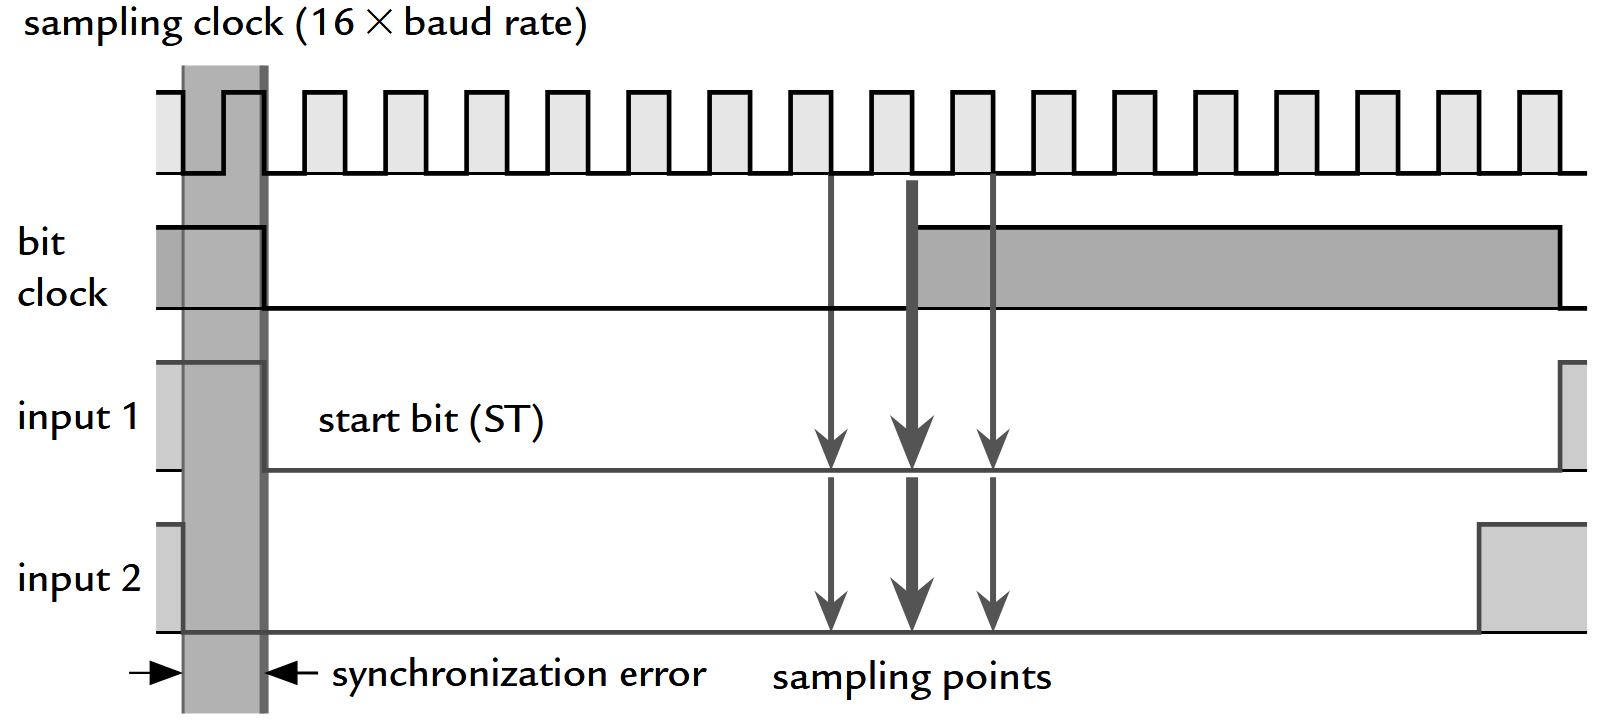
\includegraphics[width=1.0\textwidth]{../Bilder/uart_protocoll.png}
	\caption{UART \"ubertragung der Werte 0x55 und 0xFF\\\Zitat[S. 577, Abb. 10.19]{davies:msp430}}
	\label{fig:uart_uebertragung}
\end{figure}

Die interne \NeuerBegriff{Bit-Clock} (\Abkuerzung{Bit-Clock}{BITCLK}) des Empf\"angers wird mit der fallenden Flanke des eingegangenen Start-Bits synchronisiert und operiert mit der Frequenz der eingestellten Baudrate. Da die fallende Flanke des Start-Bits zu einem beliebigen Zeitpunkt relativ zur Sampling Clock auftreten kann, entsteht ein initialer Synchronisationsfehler von bis zu einer halben Periode der Sampling Clock. Die in \Abbildung{uart_uebertragung} dargestellten Szenarien, bezeichnet als \glqq Input 1\grqq und \glqq Input 2\grqq, illustrieren die hieraus resultierende minimale und maximale zeitliche Verschiebung bei der Detektion der Startbit-Flanke, abh\"angig vom Phasenverh\"altnis zwischen dem Datensignal und der Sampling Clock.\Zitat[S. 476, kap. 18.2, S. 574, Kap. 10.12 \& S. 575, Kap. 10.12.1]{ti:slau272d, davies:msp430}

\newpage
\subsubsection{Datenintegrit\"at, Fehlererkennung und weitere technischen Details}
\label{sec:datenintegritaet}

Zur Sicherstellung der Datenintegrit\"at kann eine Fehlererkennung, beispielsweise \"uber ein Parit\"atsbit, eingesetzt werden. Ein UART-Datenpaket (Frame) besteht somit typischerweise aus einem Start-Bit, sieben oder acht Datenbits, optional einem Parit\"atsbit (konfigurierbar f\"ur gerade oder ungerade Parit\"at) und einem oder (seltener) mehreren Stop-Bits. 

Die Implementierung komplexerer Fehlererkennung oder gar Fehlerkorrekturmechanismen, wie \zB Pr\"ufsummen (Checksum), obliegt \"ublicherweise der \"ubergeordneten Protokollebene, die auf der UART-Kommunikation aufsetzt. Dar\"uber hinaus ist f\"ur eine erfolgreiche Kommunikation die eindeutige Festlegung der Bitreihenfolge essentiell. Die \Abkuerzung{Least Significant Bit}{LSB}-first-Konvention ist De-facto-Standard.\Zitat[S. 574, Kap. 10.12 \& S. 575, Kap. 10.12.1]{davies:msp430}

Die Automatische Fehlererkennung des Interfaces erlaubt es dem Benutzer, schnell und ohne gro{\ss}en Implementierungsaufwand auf Grenzf\"alle und \"Ubertragungsfehler zu reagieren. \Tabelle{uart_error_flags} schl\"usselt alle wichtigen Fehler-Flags mit ihren zugeh\"origen Beschreibungen auf.

\begin{table}[h!]
	\small
	\centering
	\begin{tabular}{|l|c|p{8.5cm}|}
		\hline
		\textbf{Fehlerbedingung} & \textbf{Fehler-Flag} & \textbf{Beschreibung} \\
		\hline
		Framing-Fehler & UCFE & Tritt auf, wenn das Stoppbit nicht den erwarteten High-Pegel hat. Bei zwei Stoppbits werden beide gepr\"uft. Bei Fehler wird das UCFE-Bit gesetzt. \\\hline
		Parit\"atsfehler & UCPE & Entsteht durch eine Abweichung zwischen berechneter und tats\"achlicher Parit\"at. Adressbits werden in die Berechnung einbezogen. Bei Fehler wird UCPE gesetzt. \\\hline
		Empfangs\"uberlauf & UCOE & Wenn ein neues Zeichen empfangen wird, bevor das vorherige gelesen wurde, wird ein \"Uberlauf erkannt und das UCOE-Bit gesetzt. \\\hline
		Break-Bedingung & UCBRK & Wird erkannt, wenn alle Bits (Daten-, Parit\"ats- und Stoppbits) auf Low liegen (bei deaktivierter Baudratenerkennung). UCBRK wird gesetzt und \ggf auch UCRXIFG, wenn UCBRKIE aktiv ist. \\\hline
	\end{tabular}
	\caption{UART-Fehlerbedingungen und zugeh\"orige Status-Flags des MSP430FR5729\\\Zitat[S. 483, Tab. 18-1]{ti:slau272d}}
	\label{tab:uart_error_flags}
\end{table}

\newpage
Weitere technische Spezifikationen sind in \Tabelle{uart_features} zusammengefasst. Eine minimale Konfiguration der Schnittstelle auf den UART-Betrieb wird in \Kapitel{eUSCI_Konfiguration} detailliert beschrieben.

\begin{table}[h!]
	\small
	\centering
	\begin{tabular}{|p{6.5cm}|p{7cm}|}
		\hline
		\textbf{Funktion} & \textbf{Beschreibung} \\
		\hline
		Multiprozessor-Kommunikationsprotokolle & Unterst\"utzt integrierte Idle-Line- und Address-Bit-Protokolle f\"ur Kommunikation in Multiprozessorsystemen \\
		\hline
		Energiesparmodus-Unterst\"utzung & Startflankenerkennung (Start Edge Detection) im Empf\"anger erm\"oglicht automatisches Aufwachen aus LPMx-Modi (ausgenommen LPMx.5) \\
		\hline
		Fehlererkennung & Statusflags zur Detektion und Unterdr\"uckung von Kommunikationsfehlern (z.\,B. Framing-, Parit\"ats- oder \"uberlauffehler) \\
		\hline
		Adresserkennung & Statusflags zur Erkennung von adressierten Datenpaketen in multiprozessorf\"ahigen Systemen \\
		\hline
		Interrupt-Unterst\"utzung & Unabh\"angige Interruptquellen f\"ur Empfang, \"ubertragung, Startbit-Empfang sowie Abschluss der \"ubertragung \\
		\hline
	\end{tabular}
	\caption{Technische Merkmale der UART-Schnittstelle des MSP430FR5729\\\Zitat[S. 476, kap. 18.2]{ti:slau272d}}
	\label{tab:uart_features}
\end{table}

\subsubsection{Automatische Baudraten-Erkennung}
\label{sec:auto_baud}

Neben der Einrichtung einer statischen Baudrate kann die automatische Baudraten-Erkennung selbstst\"andig, \"uber eine \NeuerBegriff{Break/Sync Sequenz}, die vom Sender verwendete Baudrate ermitteln. Diese Synchronisations-Sequenz besteht aus einem \NeuerBegriff{Break} und einem \NeuerBegriff{Sync} Feld. Der Bereich der erkennbaren Baudraten liegt im Oversampling-Modus zwischen 244 Baud (im niedrigfrequenz-Modus beginnend ab 15 Baud) und einem Megabaud. Ein Break beinhaltet zwischen 11 und 21 \"ubertragenen Nullen, w\"ahrenddessen alle weiteren empfangenen 0en einen \NeuerBegriff{Break Timeout}-Fehler ausl\"osen. Aus Konformit\"atsgr\"unden sollte das UART Protokoll auf acht Datenbits, mit LSB-first, keiner Parit\"at und einem Stop-Bit konfiguriert werden. In \Abbildung{auto_baud} ist die beschriebene Break/Sync-Sequenz dargestellt.

\begin{figure}[h!]
	\centering
	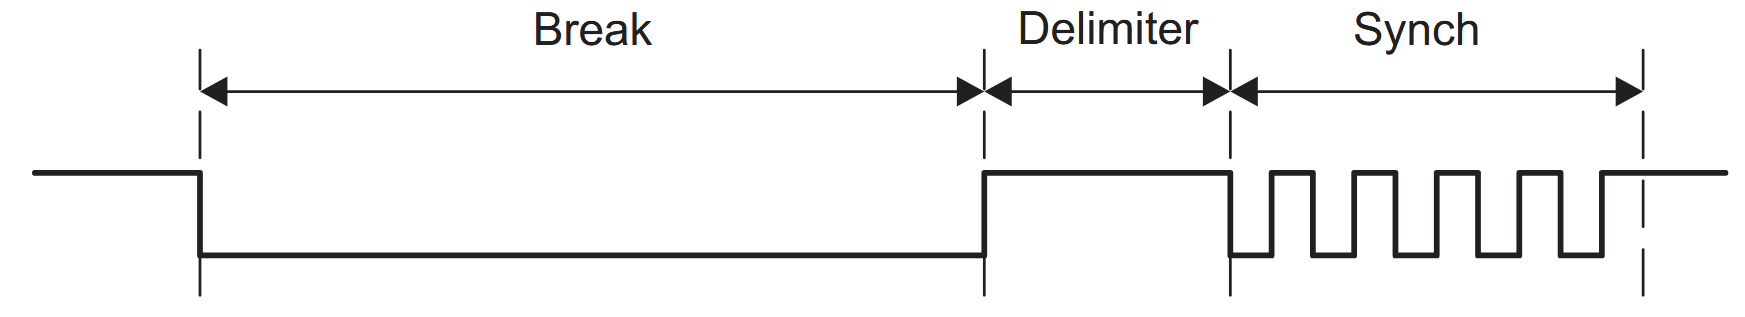
\includegraphics[width=1.0\textwidth]{../Bilder/auto_baud.png}
	\caption{Automatische Baudraten-Erkennung - Break/Sync Sequenz\\\Zitat[S. 481, Abb. 18-5]{ti:slau272d}}
	\label{fig:auto_baud}
\end{figure}

\newpage
Der Synchronisations-Prozess beginnt mit der \"Ubertragung des hexadezimalen Wertes 0x55. Die Zeit zwischen der ersten und letzten fallenden Flanke wird gemessen, um die vom Sender verwendete Baudrate zu ermitteln. Dies ist grafisch in \Abbildung{sync_field} dargestellt. Falls die maximal messbare Zeit \"uberschritten wird tritt ein \NeuerBegriff{Sync-Timeout}-Fehler auf. Falls die Messung erfolgreich war, kann nach dem setzen des \NeuerBegriff{Receive Interrupt Flags} die Information ausgelesen werden. 

Nach jedem empfangenen Zeichen ist zu beachten, das \NeuerBegriff{UCDORM}-Bit zur\"uckzusetzen, da bei gesetztem Bit zwar alle Zeichen empfangen, aber nicht in das Puffer-Register der Schnittstelle geschrieben werden. \Zitat[S. 481, Kap. 18.3.4]{ti:slau272d}

\begin{figure}[h!]
	\centering
	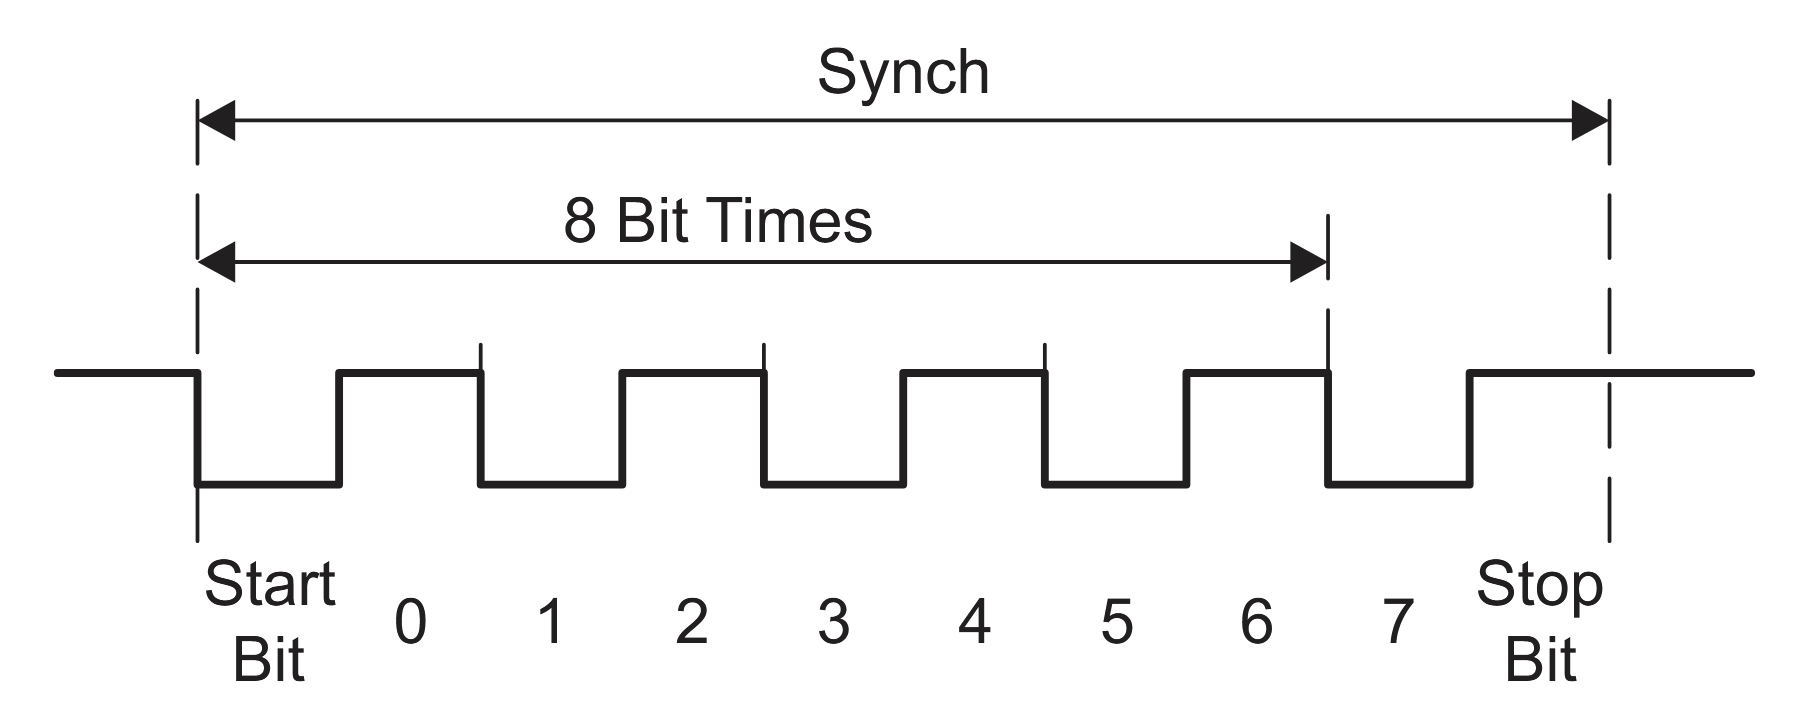
\includegraphics[width=0.95\textwidth]{../Bilder/sync_field.png}
	\caption{Automatische Baudraten-Erkennung - Sync Feld\\\Zitat[S. 481, Abb. 18-6]{ti:slau272d}}
	\label{fig:sync_field}
\end{figure}

\newpage
\subsection{eUSCI-Konfiguration}
\label{sec:eUSCI_Konfiguration}

Die Initialisierung und Konfiguration des eUSCI\_A-Moduls f\"ur den UART-Betrieb erfordert eine genaue Abfolge von Schritten zum Setzen von verschiedenen Bits und Werten in die daf\"ur vorgesehene Register. Der Prozess beginnt mit dem setzen des \Code{UCSWRST}-Bits. Dieses Bit erm\"oglicht die Konfiguration der Schnittstelle und schlie{\ss}t unerw\"unschtes Verhalten aus. Dabei wird das \Code{UCTXIFG}-Bit, zum freigeben der Konfiguration, gesetzt. Zudem werden diverse Interrupt-Enable-Bits wie \Code{UCRXIE} und \Code{UCTXIE} sowie Status- und Fehlerflags (\Code{UCRXIFG, UCRXERR, UCBRK, UCPE, UCOE, UCFE, UCSTOE, UCBTOE}) im \Code{UCAxSTATW}- und \Code{UCAxIFG}-Register gel\"oscht oder in einen definierten Anfangszustand gebracht. Dies versetzt das eUSCI\_A-Modul in einen sicheren Reset-Zustand.\Zitat[S. 478, Kap. 18.3.1]{ti:slau272d}

Nachdem das Modul sicher im Reset-Zustand initialisiert wurde, k\"onnen weitere spezifische Konfigurationsparameter f\"ur den UART-Betrieb gesetzt werden. Hierzu z\"ahlen insbesondere die folgenden Kontrollbits im \Code{UCAxCTLWn}-Register, welche die grundlegenden Betriebscharakteristika des UART-Modus definieren, wie beispielsweise:

\begin{itemize}
	\item \textbf{UCPEN:} Aktiviert die Parit\"atspr\"ufung.
	\item \textbf{UCPAR:} Festlegen einer geraden oder ungeraden Parit\"at.
	\item \textbf{UCMSB:} Legt die Bitreihenfolge fest (LSB- oder MSB-first).
	\item \textbf{UC7BIT:} Konfiguriert die Datenl\"ange auf 7 oder 8 Bit.
	\item \textbf{UCSPB:} Anzahl der Stop-Bits.
	\item \textbf{UCMODEx:} W\"ahlt den UART-Modus. (\zB 0 f\"ur Normal-Betrieb, 3 f\"ur  automatische Baudratenerkennung)
	\item \textbf{UCSYNC:} F\"ur den asynchronen UART-Betrieb muss dieses Bit auf 0 gesetzt werden.
	\item \textbf{UCSSELx:} Taktquelle f\"ur Baudratengenerator.
\end{itemize}

\newpage
\"Uber die genannten grundlegenden Einstellungen hinaus existieren weitere spezifischere Kontrollbits. Beispielsweise ist das \Code{UCRXEIE}-Bit zur freigabe des Fehler-Interrupts und das \Code{UCBRKIE} zum aktivieren der Break-Interrupts zust\"andig. Spezialfunktionen wie der Multiprozessor-Modus, welcher \"uber das \Code{UCTXADDR}-Bit gesteuert wird, oder das Senden eines Break-Zeichens mittels \Code{UCTXBRK} sind f\"ur eine Standard-UART-Konfiguration oft zu vernachl\"assigen, sofern diese Funktionalit\"aten nicht explizit gefordert sind.\Zitat[S. 495, Kap. 18.4.1 \& S. 496, Kap. 18.4.2]{ti:slau272d}

Eine weitere essenzielle Konfiguration f\"ur den UART-Betrieb ist die der Baudrate. Diese erfolgt \"uber das \Code{UCAxBRW}-Register und das \Code{UCAxMCTLW}-Register. Die korrekte Wertermittlung f\"ur diese Register ist direkt von der Frequenz der zuvor mittels \Code{UCSSELx} gew\"ahlten Taktquelle sowie der angestrebten Baudrate abh\"angig. Der Family User's Guide des MSP430FR5729 von Texas Intruments liefert f\"ur die Berechnung dieser Werte detaillierte Formeln und Beispieltabellen. Das \Code{UCAxBRW}-Register nimmt den ganzzahligen Anteil des Baudratenteilers (Prescaler) auf. Das \Code{UCAxMCTLW}-Register beinhaltet die Konfiguration f\"ur die Modulation der Frequenz, sowie das Bit zur Aktivierung des Oversampling-Modus. Durch das \Code{UCBRFx}-Bit wird, in der ersten Modulationsstufe, die Feineinstellung des Prescalers vorgenommen. In der zweiten Modulationsstufe wird durch \Code{UCBRSx} ein Modulationsmuster f\"ur die BITCLK festgelegt. Im letzten Bitfeld kann nun der Oversampling-Modus aktiviert oder deaktiviert werden.\Zitat[S. 487, Kap. 18.3.10 \& S. 497, Kap. 18.4.3, 18.4.4]{ti:slau272d}

Obwohl weitere spezifische Einstellungen m\"oglich sind, w\"urde deren detaillierte Er\"orterung den Rahmen dieser \"Ubersicht \"uberschreiten. Eine unerl\"assliche, abschlie{\ss}ende Konfigurationsma{\ss}nahme vor der Inbetriebnahme betrifft jedoch die Port-Pins: Die f\"ur den UART Betrieb verwendeten Pins m\"ussen, \"uber die Function-Select-Register (PxSEL), auf die asynchrone UART-Kommunikation konfiguriert werden. \Zitat[S. 294, Kap. 8.2.5]{ti:slau272d}

Nach Abschluss aller Konfigurationseinstellungen wird das \Code{UCSWRST}-Bit im \Code{UCAxCTLW0}-Register gel\"oscht (auf 0 zur\"uckgesetzt). Dieser Schritt hebt den Reset-Zustand auf und aktiviert das eUSCI-Modul mit der zuvor definierten Konfiguration. Optional k\"onnen nun die gew\"unschten Interrupts, wie \zB der Sende- (\Code{UCTXIE}), Empfangs- (\Code{UCRXIE}), Transmit-Complete- (\Code{UCTXCPTIE}) oder Start-Bit-Interrupt (\Code{UCSTTIE}), im \Code{UCAxIE}-Register aktiviert werden, um eine ereignisgesteuerte Datenverarbeitung zu erm\"oglichen. \Zitat[S. 502, Kap. 18.4.10]{ti:slau272d}
	
Diese sorgf\"altige Konfigurationssequenz ist entscheidend f\"ur die zuverl\"assige Funktion der UART-Schnittstelle des MSP430-Mikrocontrollers.

\subsection{Zusammenfassung}
\label{sec:eUSCI_Zusammenfassung}

Die vorangegangenen Kapitel haben die Kommunikationsschnittstelle des MSP430FR5729 im UART-Betrieb detailliert beleuchtet. Das eUSCI-Modul dient der serielle Kommunikation mit Peripherieger\"aten oder anderen Systemen. Dazu werden synchrone Protokolle wie SPI und I$^{2}$C und asynchrone Protokolle wie UART bereitgestellt.

Im Rahmen dieser Arbeit zeigte sich (siehe \Kapitel{Einordnung_Schnittstellen}), dass sich das asynchrone Kommunikationsprotokoll UART am besten f\"ur die Kommunikation zwischen dem MSP430FR5729 und einem PC-System geeignet ist. Die Bewertung der Schnittstellen erfolgte unter den Gesichtspunkten Implementierungsaufwand, Robustheit, Interruptf\"ahigkeit und Kompatibilit\"at.

Wesentliche Aspekte des UART-Betriebs ist die asynchrone Natur der Kommunikation und die wechselseitige Daten\"ubertragung zwischen zwei Parteien mittels Baudraten-Synchronisation, auch Vollduplex-Kommunikation genannt. Wichtige Merkmale hierzu ist das Datenformat (\zB acht Datenbits, LSB-first, ein SP) und die Mechanismen zur Fehlererkennung (\zB Framing-, Parity-, Overrun-Error).

Die automatische Baudraten-Erkennung erh\"oht bei der Verkn\"upfung mehrerer Kommunikationspartner \"uber dieselbe Leitung die Flexibilit\"at, steigert jedoch auch die Komplexit\"at. Da f\"ur die aktuelle Anwendung keine Verbindung mit unterschiedlichen Baudraten \"uber eine einzelne Schnittstelle erforderlich ist, wird diese Funktion nicht ben\"otigt.

Die zentralen Schritte zur Konfiguration des eUSCI-Moduls für den UART-Betrieb umfasst das Einleiten des eUSCI-Software-Resets, das Setzen und gegebenenfalls R\"ucksetzen notwendiger Steuerbits in den Kontrollregistern, die Feinabstimmung der gew\"unschten Baudrate \"uber Prescaler-Werte und schlie{\ss}lich das Aufheben des Reset-Zustandes zur Aktivierung des Moduls.

\Abbildung{BlockDiagramm_eUSCI_A_UART} zeigt ein detailliertes Blockdiagramm des eUSCI\_A-Moduls in der konfigurierten UART-Betriebsart.

\newpage
\begin{figure}[h!]
	\centering
	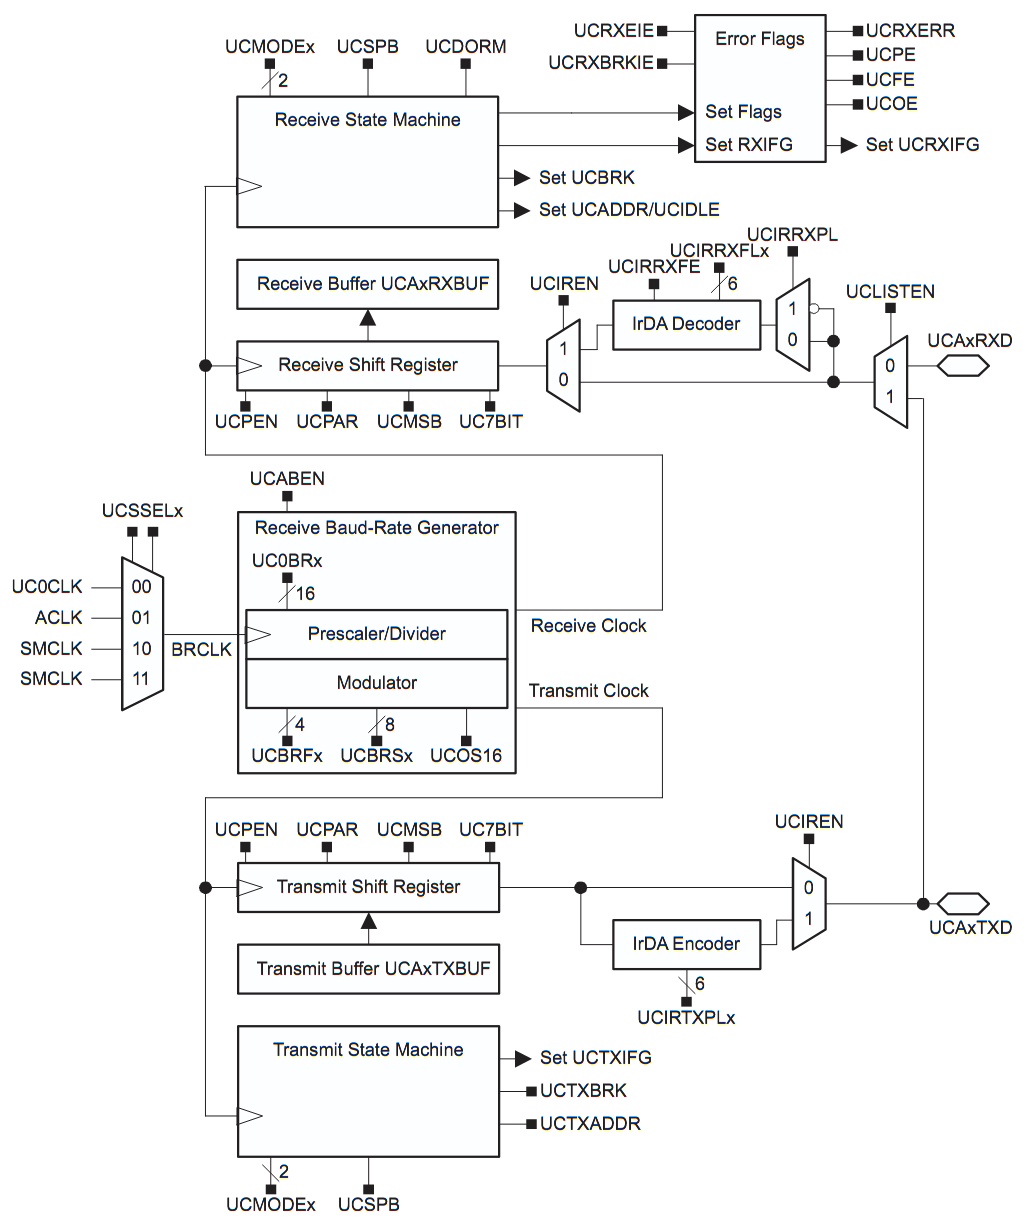
\includegraphics[width=1.0\textwidth]{../Bilder/eUSCI_UART.png}
	\caption{eUSCI Typ A -- UART-Modus\\\Zitat[S. 477, Kap. 18.2]{ti:slau272d}}
	\label{fig:BlockDiagramm_eUSCI_A_UART}
\end{figure}